% Options for packages loaded elsewhere
% Options for packages loaded elsewhere
\PassOptionsToPackage{unicode}{hyperref}
\PassOptionsToPackage{hyphens}{url}
\PassOptionsToPackage{dvipsnames,svgnames,x11names}{xcolor}
%
\documentclass[
  letterpaper,
  DIV=11,
  numbers=noendperiod]{scrreprt}
\usepackage{xcolor}
\usepackage{amsmath,amssymb}
\setcounter{secnumdepth}{5}
\usepackage{iftex}
\ifPDFTeX
  \usepackage[T1]{fontenc}
  \usepackage[utf8]{inputenc}
  \usepackage{textcomp} % provide euro and other symbols
\else % if luatex or xetex
  \usepackage{unicode-math} % this also loads fontspec
  \defaultfontfeatures{Scale=MatchLowercase}
  \defaultfontfeatures[\rmfamily]{Ligatures=TeX,Scale=1}
\fi
\usepackage{lmodern}
\ifPDFTeX\else
  % xetex/luatex font selection
\fi
% Use upquote if available, for straight quotes in verbatim environments
\IfFileExists{upquote.sty}{\usepackage{upquote}}{}
\IfFileExists{microtype.sty}{% use microtype if available
  \usepackage[]{microtype}
  \UseMicrotypeSet[protrusion]{basicmath} % disable protrusion for tt fonts
}{}
\makeatletter
\@ifundefined{KOMAClassName}{% if non-KOMA class
  \IfFileExists{parskip.sty}{%
    \usepackage{parskip}
  }{% else
    \setlength{\parindent}{0pt}
    \setlength{\parskip}{6pt plus 2pt minus 1pt}}
}{% if KOMA class
  \KOMAoptions{parskip=half}}
\makeatother
% Make \paragraph and \subparagraph free-standing
\makeatletter
\ifx\paragraph\undefined\else
  \let\oldparagraph\paragraph
  \renewcommand{\paragraph}{
    \@ifstar
      \xxxParagraphStar
      \xxxParagraphNoStar
  }
  \newcommand{\xxxParagraphStar}[1]{\oldparagraph*{#1}\mbox{}}
  \newcommand{\xxxParagraphNoStar}[1]{\oldparagraph{#1}\mbox{}}
\fi
\ifx\subparagraph\undefined\else
  \let\oldsubparagraph\subparagraph
  \renewcommand{\subparagraph}{
    \@ifstar
      \xxxSubParagraphStar
      \xxxSubParagraphNoStar
  }
  \newcommand{\xxxSubParagraphStar}[1]{\oldsubparagraph*{#1}\mbox{}}
  \newcommand{\xxxSubParagraphNoStar}[1]{\oldsubparagraph{#1}\mbox{}}
\fi
\makeatother

\usepackage{color}
\usepackage{fancyvrb}
\newcommand{\VerbBar}{|}
\newcommand{\VERB}{\Verb[commandchars=\\\{\}]}
\DefineVerbatimEnvironment{Highlighting}{Verbatim}{commandchars=\\\{\}}
% Add ',fontsize=\small' for more characters per line
\usepackage{framed}
\definecolor{shadecolor}{RGB}{241,243,245}
\newenvironment{Shaded}{\begin{snugshade}}{\end{snugshade}}
\newcommand{\AlertTok}[1]{\textcolor[rgb]{0.68,0.00,0.00}{#1}}
\newcommand{\AnnotationTok}[1]{\textcolor[rgb]{0.37,0.37,0.37}{#1}}
\newcommand{\AttributeTok}[1]{\textcolor[rgb]{0.40,0.45,0.13}{#1}}
\newcommand{\BaseNTok}[1]{\textcolor[rgb]{0.68,0.00,0.00}{#1}}
\newcommand{\BuiltInTok}[1]{\textcolor[rgb]{0.00,0.23,0.31}{#1}}
\newcommand{\CharTok}[1]{\textcolor[rgb]{0.13,0.47,0.30}{#1}}
\newcommand{\CommentTok}[1]{\textcolor[rgb]{0.37,0.37,0.37}{#1}}
\newcommand{\CommentVarTok}[1]{\textcolor[rgb]{0.37,0.37,0.37}{\textit{#1}}}
\newcommand{\ConstantTok}[1]{\textcolor[rgb]{0.56,0.35,0.01}{#1}}
\newcommand{\ControlFlowTok}[1]{\textcolor[rgb]{0.00,0.23,0.31}{\textbf{#1}}}
\newcommand{\DataTypeTok}[1]{\textcolor[rgb]{0.68,0.00,0.00}{#1}}
\newcommand{\DecValTok}[1]{\textcolor[rgb]{0.68,0.00,0.00}{#1}}
\newcommand{\DocumentationTok}[1]{\textcolor[rgb]{0.37,0.37,0.37}{\textit{#1}}}
\newcommand{\ErrorTok}[1]{\textcolor[rgb]{0.68,0.00,0.00}{#1}}
\newcommand{\ExtensionTok}[1]{\textcolor[rgb]{0.00,0.23,0.31}{#1}}
\newcommand{\FloatTok}[1]{\textcolor[rgb]{0.68,0.00,0.00}{#1}}
\newcommand{\FunctionTok}[1]{\textcolor[rgb]{0.28,0.35,0.67}{#1}}
\newcommand{\ImportTok}[1]{\textcolor[rgb]{0.00,0.46,0.62}{#1}}
\newcommand{\InformationTok}[1]{\textcolor[rgb]{0.37,0.37,0.37}{#1}}
\newcommand{\KeywordTok}[1]{\textcolor[rgb]{0.00,0.23,0.31}{\textbf{#1}}}
\newcommand{\NormalTok}[1]{\textcolor[rgb]{0.00,0.23,0.31}{#1}}
\newcommand{\OperatorTok}[1]{\textcolor[rgb]{0.37,0.37,0.37}{#1}}
\newcommand{\OtherTok}[1]{\textcolor[rgb]{0.00,0.23,0.31}{#1}}
\newcommand{\PreprocessorTok}[1]{\textcolor[rgb]{0.68,0.00,0.00}{#1}}
\newcommand{\RegionMarkerTok}[1]{\textcolor[rgb]{0.00,0.23,0.31}{#1}}
\newcommand{\SpecialCharTok}[1]{\textcolor[rgb]{0.37,0.37,0.37}{#1}}
\newcommand{\SpecialStringTok}[1]{\textcolor[rgb]{0.13,0.47,0.30}{#1}}
\newcommand{\StringTok}[1]{\textcolor[rgb]{0.13,0.47,0.30}{#1}}
\newcommand{\VariableTok}[1]{\textcolor[rgb]{0.07,0.07,0.07}{#1}}
\newcommand{\VerbatimStringTok}[1]{\textcolor[rgb]{0.13,0.47,0.30}{#1}}
\newcommand{\WarningTok}[1]{\textcolor[rgb]{0.37,0.37,0.37}{\textit{#1}}}

\usepackage{longtable,booktabs,array}
\usepackage{calc} % for calculating minipage widths
% Correct order of tables after \paragraph or \subparagraph
\usepackage{etoolbox}
\makeatletter
\patchcmd\longtable{\par}{\if@noskipsec\mbox{}\fi\par}{}{}
\makeatother
% Allow footnotes in longtable head/foot
\IfFileExists{footnotehyper.sty}{\usepackage{footnotehyper}}{\usepackage{footnote}}
\makesavenoteenv{longtable}
\usepackage{graphicx}
\makeatletter
\newsavebox\pandoc@box
\newcommand*\pandocbounded[1]{% scales image to fit in text height/width
  \sbox\pandoc@box{#1}%
  \Gscale@div\@tempa{\textheight}{\dimexpr\ht\pandoc@box+\dp\pandoc@box\relax}%
  \Gscale@div\@tempb{\linewidth}{\wd\pandoc@box}%
  \ifdim\@tempb\p@<\@tempa\p@\let\@tempa\@tempb\fi% select the smaller of both
  \ifdim\@tempa\p@<\p@\scalebox{\@tempa}{\usebox\pandoc@box}%
  \else\usebox{\pandoc@box}%
  \fi%
}
% Set default figure placement to htbp
\def\fps@figure{htbp}
\makeatother





\setlength{\emergencystretch}{3em} % prevent overfull lines

\providecommand{\tightlist}{%
  \setlength{\itemsep}{0pt}\setlength{\parskip}{0pt}}



 


\KOMAoption{captions}{tableheading}
\makeatletter
\@ifpackageloaded{bookmark}{}{\usepackage{bookmark}}
\makeatother
\makeatletter
\@ifpackageloaded{caption}{}{\usepackage{caption}}
\AtBeginDocument{%
\ifdefined\contentsname
  \renewcommand*\contentsname{Table of contents}
\else
  \newcommand\contentsname{Table of contents}
\fi
\ifdefined\listfigurename
  \renewcommand*\listfigurename{List of Figures}
\else
  \newcommand\listfigurename{List of Figures}
\fi
\ifdefined\listtablename
  \renewcommand*\listtablename{List of Tables}
\else
  \newcommand\listtablename{List of Tables}
\fi
\ifdefined\figurename
  \renewcommand*\figurename{Figure}
\else
  \newcommand\figurename{Figure}
\fi
\ifdefined\tablename
  \renewcommand*\tablename{Table}
\else
  \newcommand\tablename{Table}
\fi
}
\@ifpackageloaded{float}{}{\usepackage{float}}
\floatstyle{ruled}
\@ifundefined{c@chapter}{\newfloat{codelisting}{h}{lop}}{\newfloat{codelisting}{h}{lop}[chapter]}
\floatname{codelisting}{Listing}
\newcommand*\listoflistings{\listof{codelisting}{List of Listings}}
\makeatother
\makeatletter
\makeatother
\makeatletter
\@ifpackageloaded{caption}{}{\usepackage{caption}}
\@ifpackageloaded{subcaption}{}{\usepackage{subcaption}}
\makeatother
\usepackage{bookmark}
\IfFileExists{xurl.sty}{\usepackage{xurl}}{} % add URL line breaks if available
\urlstyle{same}
\hypersetup{
  pdftitle={K-Means Clustering \& Bofedales},
  pdfauthor={Estella Newton},
  colorlinks=true,
  linkcolor={blue},
  filecolor={Maroon},
  citecolor={Blue},
  urlcolor={Blue},
  pdfcreator={LaTeX via pandoc}}


\title{K-Means Clustering \& Bofedales}
\author{Estella Newton}
\date{2025-07-10}
\begin{document}
\maketitle

\renewcommand*\contentsname{Table of contents}
{
\hypersetup{linkcolor=}
\setcounter{tocdepth}{2}
\tableofcontents
}

\bookmarksetup{startatroot}

\chapter*{Introduction}\label{introduction}
\addcontentsline{toc}{chapter}{Introduction}

\markboth{Introduction}{Introduction}

\section*{What are bofedales?}\label{what-are-bofedales}
\addcontentsline{toc}{section}{What are bofedales?}

\markright{What are bofedales?}

Bofedales are unique high-Andean wetland ecosystems characterized by
peat formation. Located over 3,000m above sea level, they originate due
to permanent water flows that foster the development of cushion plants.
Cushion-forming Juncaceae are ``nurse plants'' for plants consumed by
wild and domesticated camelids. Bofedales are essential for water
management, have high cultural value for indigenous communities
(especially herders and farmers), and play a key role in the global
climate systems. They can be found in Peru, Bolivia, and northern Chile,
the region focused on by this study.

\section*{What is a k-means clustering
algorithm?}\label{what-is-a-k-means-clustering-algorithm}
\addcontentsline{toc}{section}{What is a k-means clustering algorithm?}

\markright{What is a k-means clustering algorithm?}

K-means clustering is a type of unsupervised machine learning model. If
all of the n features of the dataset were graphed in a n-dimensional
space, k-means attempts to create a set of centers and minimize the sum
of squared distances between any point and its center. Since this
problem is NP-hard, k-means is a heuristic algorithm that converges as a
local optimum.

\begin{center}\rule{0.5\linewidth}{0.5pt}\end{center}

This project is part of the Núcleo Milenio Andespeat, a research center
funded by ANID and based at the Universidad de Tarapacá in Arica, Chile.
It was developed by Estella Newton and advised by Manuel Prieto, Charlie
Hoffs, and Francisco Mayol.

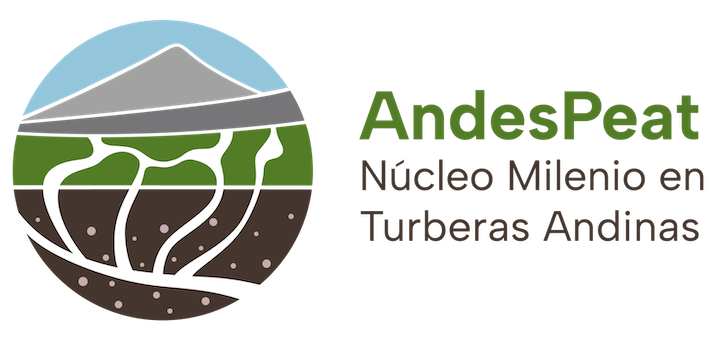
\includegraphics[width=\linewidth,height=0.83333in,keepaspectratio]{images/AndesPeatLogo.png}
~

\includegraphics[width=\linewidth,height=0.83333in,keepaspectratio]{images/UniversityOfTarapacaLogo.png}
~

\includegraphics[width=\linewidth,height=0.83333in,keepaspectratio]{images/ANIDLogo.png}

\bookmarksetup{startatroot}

\chapter{Research Questions \&
Objectives}\label{research-questions-objectives}

\section{Research Question}\label{research-question}

\subsection{Main Question}\label{main-question}

What can a machine learning algorithm reveal about the impact of various
factors on the health of bofedales in Chile?

\subsection{Sub-Questions}\label{sub-questions}

\begin{enumerate}
\def\labelenumi{\arabic{enumi}.}
\tightlist
\item
  What models are effective for analyzing the impact of various factors
  on the health of bofedales in Chile?
\item
  What factors prove most influential to the health of bofedales in
  Chile based on available data?
\item
  What can the clusters produced by the model reveal about Chilean
  bofedal health?
\end{enumerate}

\section{Research Objectives}\label{research-objectives}

\subsection{Main Objective}\label{main-objective}

Build and train several different machine learning algorithms on various
factors that may affect Chilean bofedal health.

\subsection{Sub-Objectives}\label{sub-objectives}

\begin{enumerate}
\def\labelenumi{\arabic{enumi}.}
\tightlist
\item
  Determine which types of ML algorithms best reveal impacts to bofedal
  health.
\item
  Interpret the weights given to each variable by the ML model.
\item
  Analyze clusters to determine the meaning of each cluster and its
  typical attributes.
\end{enumerate}

\bookmarksetup{startatroot}

\chapter{Datasets \& Variables}\label{datasets-variables}

\section{The CAMELS-CL dataset}\label{the-camels-cl-dataset}

\begin{itemize}
\tightlist
\item
  Minimum Temperature
\item
  Maximum Temperature
\item
  Precipitation
\item
  Ground Water Rights
\item
  Surface Water Rights
\item
  PET
\end{itemize}

These datasets have temporal data, beginning around 1980 and ending
around 2020 (depending on the dataset)

Link to the CAMELS-CL dataset:
\href{URL}{https://doi.pangaea.de/10.1594/PANGAEA.894885}

\emph{Note: The CAMELS-CL dataset does include streamflow data, but due
to large amounts of missing data, it was not incorporated into the
model}

\section{Extracted from Sentinel-2 Satellite Imagery from
GEE}\label{extracted-from-sentinel-2-satellite-imagery-from-gee}

\begin{itemize}
\tightlist
\item
  NDVI
\item
  NDWI
\end{itemize}

Link to the Sentinel-2 dataset:
\href{URL}{https://dataspace.copernicus.eu/explore-data/data-collections/sentinel-data/sentinel-2}

These datasets have temporal data from 2019 to 2024

\section{OpenTopography's API
service}\label{opentopographys-api-service}

\begin{itemize}
\tightlist
\item
  Elevation
\item
  Elevation standard deviation
\end{itemize}

Link to OpenTopography's website:
\href{URL}{https://opentopography.org/}

\section{DGA datasets}\label{dga-datasets}

\begin{itemize}
\tightlist
\item
  Number of reservoirs
\end{itemize}

Link to download:
\href{URL}{https://dga.mop.gob.cl/uploads/sites/13/2024/07/Embalses-1.zip}

\section{Development of Groundwater Levels Dataset for Chile since 1970
publication in
Nature}\label{development-of-groundwater-levels-dataset-for-chile-since-1970-publication-in-nature}

\begin{itemize}
\tightlist
\item
  Number of boreholes/wells
\end{itemize}

Link to the publication:
\href{URL}{https://www.nature.com/articles/s41597-023-02895-5}

\section{MapBiomas}\label{mapbiomas}

\begin{itemize}
\tightlist
\item
  Protected/park land data (m\^{}2 and percentage of whole)
\end{itemize}

Link to MapBiomas:
\href{URL}{https://chile.mapbiomas.org/en/mapas-de-la-coleccion/}

\section{Variables not included}\label{variables-not-included}

Several variables that are important for consideration when examining
factors that determine overall health of a bofedal but do not have
readily avalible datasets include:

\begin{itemize}
\tightlist
\item
  Bofedal management strategies
\item
  Population dynamics in herding communities
\item
  Carrying capacity of ganandos by species
\end{itemize}

Socioeconomic variables such as these are addressed later in the study
through case studies and field work.

\part{Running K-Means}

\chapter{Principle Component
Analysis}\label{principle-component-analysis}

Since the merge between the datasets created a lot of columns (over
2,000), it's necesary to reduce the dimensions of the dataset with PCA
before running the k-means algorithm.

\section{Import Statements}\label{import-statements}

\begin{Shaded}
\begin{Highlighting}[]
\ImportTok{from}\NormalTok{ sklearn.decomposition }\ImportTok{import}\NormalTok{ PCA}
\ImportTok{from}\NormalTok{ sklearn.preprocessing }\ImportTok{import}\NormalTok{ StandardScaler}
\ImportTok{import}\NormalTok{ pandas }\ImportTok{as}\NormalTok{ pd}
\ImportTok{import}\NormalTok{ numpy }\ImportTok{as}\NormalTok{ np}
\ImportTok{import}\NormalTok{ matplotlib.pyplot }\ImportTok{as}\NormalTok{ plt}
\end{Highlighting}
\end{Shaded}

\begin{Shaded}
\begin{Highlighting}[]
\NormalTok{df }\OperatorTok{=}\NormalTok{ pd.read\_csv(}\StringTok{"bofedales{-}clean.csv"}\NormalTok{)}
\NormalTok{df }\OperatorTok{=}\NormalTok{ df.drop([}\StringTok{"Unnamed: 0"}\NormalTok{], axis}\OperatorTok{=}\DecValTok{1}\NormalTok{)}
\NormalTok{df.isna().}\BuiltInTok{sum}\NormalTok{().}\BuiltInTok{sum}\NormalTok{()}
\end{Highlighting}
\end{Shaded}

\begin{verbatim}
np.int64(0)
\end{verbatim}

\begin{Shaded}
\begin{Highlighting}[]
\NormalTok{df.shape}
\end{Highlighting}
\end{Shaded}

\begin{verbatim}
(2534, 2289)
\end{verbatim}

\begin{Shaded}
\begin{Highlighting}[]
\NormalTok{df.head(}\DecValTok{3}\NormalTok{)}
\end{Highlighting}
\end{Shaded}

\begin{longtable}[]{@{}llllllllllllllllllllll@{}}
\toprule\noalign{}
& Area\_m2 & AUC & pct\_prot & elev\_mean\_ & elev\_std\_m & n\_wells &
Ground Water Rights 1966-01-01 & Ground Water Rights 1967-01-01 & Ground
Water Rights 1968-01-01 & Ground Water Rights 1969-01-01 & ... & NDWI
2019-03 & NDWI 2019-04 & NDWI 2019-05 & NDWI 2019-06 & NDWI 2019-07 &
NDWI 2019-08 & NDWI 2019-09 & NDWI 2019-10 & NDWI 2019-11 & NDWI
2019-12 \\
\midrule\noalign{}
\endhead
\bottomrule\noalign{}
\endlastfoot
0 & 6300 & 86.769539 & 0.0 & 4162.714286 & 3.953815 & 0.0 & 0.0 & 0.0 &
0.0 & 0.0 & ... & 0.031930 & 0.026136 & 0.022087 & 0.019181 & 0.023405 &
0.015355 & -0.000504 & 0.004056 & 0.014678 & 0.010436 \\
1 & 5400 & 83.176353 & 0.0 & 4073.500000 & 12.406316 & 0.0 & 0.0 & 0.0 &
0.0 & 0.0 & ... & -0.057992 & -0.053230 & -0.054671 & -0.064990 &
-0.063351 & -0.074670 & -0.085071 & -0.081491 & -0.061333 & -0.055450 \\
2 & 6300 & 103.719438 & 0.0 & 4278.571429 & 6.161102 & 0.0 & 0.0 & 0.0 &
0.0 & 0.0 & ... & 0.065899 & 0.070822 & 0.070075 & 0.068015 & 0.068144 &
0.062340 & 0.047670 & 0.050570 & 0.056227 & 0.059294 \\
\end{longtable}

\section{Finding the Optimal Number of Principle
Components}\label{finding-the-optimal-number-of-principle-components}

First, check how many principle components account for 90\% of the
variance in the data

\begin{Shaded}
\begin{Highlighting}[]
\NormalTok{scaler }\OperatorTok{=}\NormalTok{ StandardScaler()}
\NormalTok{X\_scaled }\OperatorTok{=}\NormalTok{ scaler.fit\_transform(df)  }
\end{Highlighting}
\end{Shaded}

\begin{Shaded}
\begin{Highlighting}[]
\NormalTok{x\_per\_variance }\OperatorTok{=} \FloatTok{0.90}

\NormalTok{pca }\OperatorTok{=}\NormalTok{ PCA(n\_components}\OperatorTok{=}\NormalTok{x\_per\_variance, svd\_solver}\OperatorTok{=}\StringTok{"full"}\NormalTok{)}
\NormalTok{X\_pca }\OperatorTok{=}\NormalTok{ pca.fit\_transform(X\_scaled)}
\BuiltInTok{print}\NormalTok{(}\SpecialStringTok{f"Number of principal components chosen to explain }\SpecialCharTok{\{}\NormalTok{x\_per\_variance }\OperatorTok{*} \DecValTok{100}\SpecialCharTok{\}}\SpecialStringTok{\% variance: }\SpecialCharTok{\{}\NormalTok{pca}\SpecialCharTok{.}\NormalTok{n\_components\_}\SpecialCharTok{\}}\SpecialStringTok{"}\NormalTok{)}
\BuiltInTok{print}\NormalTok{(}\StringTok{"Explained variance ratio (per PC):"}\NormalTok{)}
\BuiltInTok{print}\NormalTok{(np.}\BuiltInTok{round}\NormalTok{(pca.explained\_variance\_ratio\_, }\DecValTok{4}\NormalTok{))}
\BuiltInTok{print}\NormalTok{(}\StringTok{"Cumulative explained variance:"}\NormalTok{, }\BuiltInTok{round}\NormalTok{(pca.explained\_variance\_ratio\_.cumsum()[}\OperatorTok{{-}}\DecValTok{1}\NormalTok{], }\DecValTok{4}\NormalTok{))}
\end{Highlighting}
\end{Shaded}

\begin{verbatim}
Number of principal components chosen to explain 90.0% variance: 5
Explained variance ratio (per PC):
[0.7058 0.0929 0.0571 0.0397 0.0334]
Cumulative explained variance: 0.9289
\end{verbatim}

Five PCs account for 90\% of the variance, so the data can easily be
greatly reduced in dimensionality.

Next, graph variance versus PCs. The elbow in the graph has the optional
number of PCs -- afterwards, there are diminishing returns.

\begin{Shaded}
\begin{Highlighting}[]
\NormalTok{features\_for\_pca }\OperatorTok{=}\NormalTok{ df.columns.tolist()}

\NormalTok{pca\_full }\OperatorTok{=}\NormalTok{ PCA()}
\NormalTok{pca\_full.fit(X\_scaled)}

\NormalTok{cum\_var }\OperatorTok{=}\NormalTok{ np.cumsum(pca\_full.explained\_variance\_ratio\_)}

\CommentTok{\# 6) Plot the "elbow" (cumulative explained variance vs. number of components)}
\NormalTok{plt.figure(figsize}\OperatorTok{=}\NormalTok{(}\DecValTok{8}\NormalTok{, }\DecValTok{5}\NormalTok{))}
\NormalTok{plt.plot(}\BuiltInTok{range}\NormalTok{(}\DecValTok{1}\NormalTok{, }\BuiltInTok{len}\NormalTok{(cum\_var) }\OperatorTok{+} \DecValTok{1}\NormalTok{), cum\_var, marker}\OperatorTok{=}\StringTok{\textquotesingle{}o\textquotesingle{}}\NormalTok{, linewidth}\OperatorTok{=}\DecValTok{2}\NormalTok{)}
\NormalTok{plt.axhline(y}\OperatorTok{=}\FloatTok{0.90}\NormalTok{, color}\OperatorTok{=}\StringTok{\textquotesingle{}r\textquotesingle{}}\NormalTok{, linestyle}\OperatorTok{=}\StringTok{\textquotesingle{}{-}{-}\textquotesingle{}}\NormalTok{, label}\OperatorTok{=}\StringTok{\textquotesingle{}90\% Threshold\textquotesingle{}}\NormalTok{)}
\NormalTok{plt.axhline(y}\OperatorTok{=}\FloatTok{0.99}\NormalTok{, color}\OperatorTok{=}\StringTok{\textquotesingle{}g\textquotesingle{}}\NormalTok{, linestyle}\OperatorTok{=}\StringTok{\textquotesingle{}{-}{-}\textquotesingle{}}\NormalTok{, label}\OperatorTok{=}\StringTok{\textquotesingle{}99\% Threshold\textquotesingle{}}\NormalTok{)}
\NormalTok{plt.xlabel(}\StringTok{"Number of Principal Components"}\NormalTok{)}
\NormalTok{plt.ylabel(}\StringTok{"Cumulative Explained Variance"}\NormalTok{)}
\NormalTok{plt.title(}\StringTok{"Elbow Plot: Cumulative Explained Variance by Number of PCs"}\NormalTok{)}
\NormalTok{plt.legend()}
\NormalTok{plt.grid(}\VariableTok{True}\NormalTok{)}
\NormalTok{plt.tight\_layout()}

\NormalTok{plt.xlim(}\DecValTok{1}\NormalTok{, }\DecValTok{50}\NormalTok{)}

\NormalTok{plt.show()}
\end{Highlighting}
\end{Shaded}

\pandocbounded{\includegraphics[keepaspectratio]{Notebooks/PCA_files/figure-pdf/cell-8-output-1.png}}

Since the ``elbow'' of the curve occurs at around 7 or 6 PCs, this is
the value that will be used in analyzing the data

\section{Run PCA with 6 Components}\label{run-pca-with-6-components}

\begin{Shaded}
\begin{Highlighting}[]
\NormalTok{pca6 }\OperatorTok{=}\NormalTok{ PCA(n\_components}\OperatorTok{=}\DecValTok{6}\NormalTok{)}
\NormalTok{X\_ }\OperatorTok{=}\NormalTok{ pca6.fit\_transform(X\_scaled)}
\end{Highlighting}
\end{Shaded}

Save the dataset to be run in future notebooks:

\begin{Shaded}
\begin{Highlighting}[]
\NormalTok{np.save(}\StringTok{"scaled{-}df.npy"}\NormalTok{, X\_)}
\end{Highlighting}
\end{Shaded}

\chapter{Running k=7}\label{running-k7}

Since the merge between the datasets created a lot of columns (over
2,000), it's necesary to reduce the dimensions of the dataset with PCA
before running the k-means algorithm.

\section{Import Statements}\label{import-statements-1}

\begin{Shaded}
\begin{Highlighting}[]
\ImportTok{from}\NormalTok{ sklearn.cluster }\ImportTok{import}\NormalTok{ KMeans}
\ImportTok{from}\NormalTok{ sklearn.metrics }\ImportTok{import}\NormalTok{ silhouette\_score, calinski\_harabasz\_score, davies\_bouldin\_score, pairwise\_distances\_argmin\_min, silhouette\_samples}

\ImportTok{import}\NormalTok{ pandas }\ImportTok{as}\NormalTok{ pd}
\ImportTok{import}\NormalTok{ numpy }\ImportTok{as}\NormalTok{ np}
\ImportTok{import}\NormalTok{ matplotlib.pyplot }\ImportTok{as}\NormalTok{ plt}
\ImportTok{import}\NormalTok{ plotly.graph\_objects }\ImportTok{as}\NormalTok{ go}

\ImportTok{import}\NormalTok{ geopandas }\ImportTok{as}\NormalTok{ gpd}
\ImportTok{from}\NormalTok{ shapely.geometry }\ImportTok{import}\NormalTok{ Point}
\ImportTok{import}\NormalTok{ contextily }\ImportTok{as}\NormalTok{ ctx}
\ImportTok{import}\NormalTok{ folium}

\ImportTok{from}\NormalTok{ matplotlib.lines }\ImportTok{import}\NormalTok{ Line2D}
\ImportTok{import}\NormalTok{ matplotlib.dates }\ImportTok{as}\NormalTok{ mdates}
\ImportTok{import}\NormalTok{ matplotlib.lines }\ImportTok{as}\NormalTok{ mlines}
\ImportTok{import}\NormalTok{ matplotlib.colors }\ImportTok{as}\NormalTok{ mcolors}
\ImportTok{import}\NormalTok{ matplotlib.cm }\ImportTok{as}\NormalTok{ cm}

\ImportTok{import}\NormalTok{ ipywidgets }\ImportTok{as}\NormalTok{ widgets}
\ImportTok{from}\NormalTok{ ipywidgets }\ImportTok{import}\NormalTok{ interact, interactive}

\ImportTok{from}\NormalTok{ sklearn.tree }\ImportTok{import}\NormalTok{ DecisionTreeClassifier}
\ImportTok{from}\NormalTok{ sklearn }\ImportTok{import}\NormalTok{ tree}
\end{Highlighting}
\end{Shaded}

\begin{Shaded}
\begin{Highlighting}[]
\NormalTok{X\_ }\OperatorTok{=}\NormalTok{ np.load(}\StringTok{"scaled{-}df.npy"}\NormalTok{)}
\NormalTok{df }\OperatorTok{=}\NormalTok{ pd.read\_csv(}\StringTok{"bofedales{-}clean.csv"}\NormalTok{)}
\end{Highlighting}
\end{Shaded}

The K-Means algorithm will run on the dataset in PC space.

\section{Find the Optional Amount of Groups for
K-Means}\label{find-the-optional-amount-of-groups-for-k-means}

\begin{Shaded}
\begin{Highlighting}[]
\NormalTok{inertias }\OperatorTok{=}\NormalTok{ []}
\NormalTok{K\_candidates }\OperatorTok{=} \BuiltInTok{list}\NormalTok{(}\BuiltInTok{range}\NormalTok{(}\DecValTok{2}\NormalTok{, }\DecValTok{15}\NormalTok{))}

\ControlFlowTok{for}\NormalTok{ k }\KeywordTok{in}\NormalTok{ K\_candidates:}
\NormalTok{    km }\OperatorTok{=}\NormalTok{ KMeans(n\_clusters}\OperatorTok{=}\NormalTok{k, random\_state}\OperatorTok{=}\DecValTok{42}\NormalTok{, n\_init}\OperatorTok{=}\DecValTok{10}\NormalTok{)}
\NormalTok{    km.fit(X\_)}
\NormalTok{    inertias.append(km.inertia\_)}

\NormalTok{plt.figure(figsize}\OperatorTok{=}\NormalTok{(}\DecValTok{6}\NormalTok{, }\DecValTok{4}\NormalTok{))}
\NormalTok{plt.plot(K\_candidates, inertias, marker}\OperatorTok{=}\StringTok{\textquotesingle{}o\textquotesingle{}}\NormalTok{, lw}\OperatorTok{=}\DecValTok{2}\NormalTok{)}
\NormalTok{plt.xlabel(}\StringTok{"Number of clusters K"}\NormalTok{)}
\NormalTok{plt.ylabel(}\StringTok{"KMeans inertia (sum of squared distances)"}\NormalTok{)}
\NormalTok{plt.title(}\StringTok{"Elbow Method on 6{-}PC data"}\NormalTok{)}
\NormalTok{plt.grid(}\VariableTok{True}\NormalTok{)}
\NormalTok{plt.show()}
\end{Highlighting}
\end{Shaded}

\pandocbounded{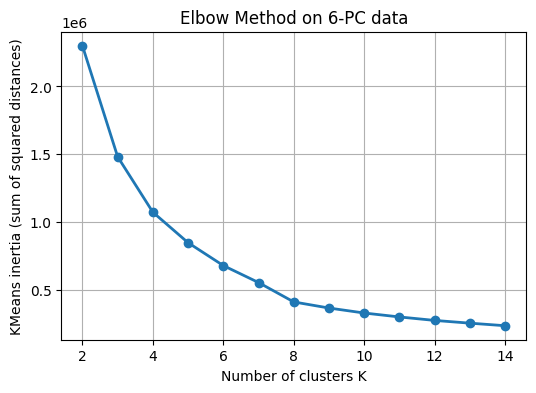
\includegraphics[keepaspectratio]{Notebooks/k7_files/figure-pdf/cell-4-output-1.png}}

From the graph, it looks like around 5-7 is the optional k value.
However, k=2 is also an optimal value.

\begin{Shaded}
\begin{Highlighting}[]
\KeywordTok{def}\NormalTok{ kmeans\_metrics(X, k\_min}\OperatorTok{=}\DecValTok{2}\NormalTok{, k\_max}\OperatorTok{=}\DecValTok{15}\NormalTok{, random\_state}\OperatorTok{=}\DecValTok{42}\NormalTok{):}
\NormalTok{    rows }\OperatorTok{=}\NormalTok{ []}
    \ControlFlowTok{for}\NormalTok{ k }\KeywordTok{in} \BuiltInTok{range}\NormalTok{(k\_min, k\_max }\OperatorTok{+} \DecValTok{1}\NormalTok{):}
\NormalTok{        km }\OperatorTok{=}\NormalTok{ KMeans(n\_clusters}\OperatorTok{=}\NormalTok{k, random\_state}\OperatorTok{=}\NormalTok{random\_state, n\_init}\OperatorTok{=}\StringTok{"auto"}\NormalTok{)}
\NormalTok{        labels }\OperatorTok{=}\NormalTok{ km.fit\_predict(X)}

\NormalTok{        rows.append(}
\NormalTok{            \{}
                \StringTok{"k"}\NormalTok{: k,}
                \StringTok{"silhouette"}\NormalTok{: silhouette\_score(X, labels),}
                \StringTok{"davies\_bouldin"}\NormalTok{: davies\_bouldin\_score(X, labels),}
                \StringTok{"calinski\_harabasz"}\NormalTok{: calinski\_harabasz\_score(X, labels),}
\NormalTok{            \}}
\NormalTok{        )}

    \ControlFlowTok{return}\NormalTok{ pd.DataFrame(rows)}


\NormalTok{results }\OperatorTok{=}\NormalTok{ kmeans\_metrics(X\_, k\_min}\OperatorTok{=}\DecValTok{2}\NormalTok{, k\_max}\OperatorTok{=}\DecValTok{14}\NormalTok{)}
\BuiltInTok{print}\NormalTok{(results)}

\CommentTok{\# Highlight the “best” K by each metric}
\NormalTok{best\_k\_sil }\OperatorTok{=}\NormalTok{ results.loc[results[}\StringTok{"silhouette"}\NormalTok{].idxmax(), }\StringTok{"k"}\NormalTok{]}
\NormalTok{best\_k\_db  }\OperatorTok{=}\NormalTok{ results.loc[results[}\StringTok{"davies\_bouldin"}\NormalTok{].idxmin(), }\StringTok{"k"}\NormalTok{]}
\NormalTok{best\_k\_ch  }\OperatorTok{=}\NormalTok{ results.loc[results[}\StringTok{"calinski\_harabasz"}\NormalTok{].idxmax(), }\StringTok{"k"}\NormalTok{]}

\BuiltInTok{print}\NormalTok{(}
    \SpecialStringTok{f"}\CharTok{\textbackslash{}n}\SpecialStringTok{Best{-}by{-}metric suggestions:}\CharTok{\textbackslash{}n}\SpecialStringTok{"}
    \SpecialStringTok{f"  • Silhouette         ➜ K = }\SpecialCharTok{\{}\NormalTok{best\_k\_sil}\SpecialCharTok{\}}\CharTok{\textbackslash{}n}\SpecialStringTok{"}
    \SpecialStringTok{f"  • Davies{-}Bouldin (↓) ➜ K = }\SpecialCharTok{\{}\NormalTok{best\_k\_db}\SpecialCharTok{\}}\CharTok{\textbackslash{}n}\SpecialStringTok{"}
    \SpecialStringTok{f"  • Calinski{-}Harabasz  ➜ K = }\SpecialCharTok{\{}\NormalTok{best\_k\_ch}\SpecialCharTok{\}}\SpecialStringTok{"}
\NormalTok{)}
\end{Highlighting}
\end{Shaded}

\begin{verbatim}
     k  silhouette  davies_bouldin  calinski_harabasz
0    2    0.704250        0.268098        2791.480831
1    3    0.490419        0.658522        3178.371016
2    4    0.451653        0.866476        3456.097292
3    5    0.462684        0.873393        3445.233408
4    6    0.487050        0.807228        3559.362944
5    7    0.480572        0.741292        3690.915274
6    8    0.544377        0.714926        4381.382113
7    9    0.488916        0.693168        4233.595603
8   10    0.495985        0.804549        4286.893976
9   11    0.498417        0.784347        4326.286214
10  12    0.488947        0.784427        4235.420425
11  13    0.465013        0.815752        3995.008086
12  14    0.466522        0.820545        4087.451788

Best-by-metric suggestions:
  • Silhouette         ➜ K = 2
  • Davies-Bouldin (↓) ➜ K = 2
  • Calinski-Harabasz  ➜ K = 8
\end{verbatim}

This notebook will run k=7 in accordance with the Calinski-Harabasz
metric and the elbow method. However, we will run k=2 in the following
chapter.

\section{Run K-Means with k=7}\label{run-k-means-with-k7}

\begin{Shaded}
\begin{Highlighting}[]
\NormalTok{K}\OperatorTok{=}\DecValTok{7}
\NormalTok{kmeans }\OperatorTok{=}\NormalTok{ KMeans(n\_clusters}\OperatorTok{=}\NormalTok{K, random\_state}\OperatorTok{=}\DecValTok{42}\NormalTok{, n\_init}\OperatorTok{=}\DecValTok{20}\NormalTok{)}
\NormalTok{cluster\_labels }\OperatorTok{=}\NormalTok{ kmeans.fit\_predict(X\_)}
\NormalTok{centroids\_pca }\OperatorTok{=}\NormalTok{ kmeans.cluster\_centers\_ }
\NormalTok{df[}\StringTok{"cluster"}\NormalTok{] }\OperatorTok{=}\NormalTok{ cluster\_labels}
\end{Highlighting}
\end{Shaded}

\begin{Shaded}
\begin{Highlighting}[]
\NormalTok{cluster\_means }\OperatorTok{=}\NormalTok{ df.groupby(}\StringTok{"cluster"}\NormalTok{).mean().}\BuiltInTok{round}\NormalTok{(}\DecValTok{2}\NormalTok{)}
\NormalTok{cluster\_means.drop(}\StringTok{"Unnamed: 0"}\NormalTok{, axis}\OperatorTok{=}\DecValTok{1}\NormalTok{, inplace}\OperatorTok{=}\VariableTok{True}\NormalTok{)}
\NormalTok{cluster\_means}
\end{Highlighting}
\end{Shaded}

\begin{longtable}[]{@{}llllllllllllllllllllll@{}}
\toprule\noalign{}
& Area\_m2 & AUC & pct\_prot & elev\_mean\_ & elev\_std\_m & n\_wells &
Ground Water Rights 1966-01-01 & Ground Water Rights 1967-01-01 & Ground
Water Rights 1968-01-01 & Ground Water Rights 1969-01-01 & ... & NDWI
2019-03 & NDWI 2019-04 & NDWI 2019-05 & NDWI 2019-06 & NDWI 2019-07 &
NDWI 2019-08 & NDWI 2019-09 & NDWI 2019-10 & NDWI 2019-11 & NDWI
2019-12 \\
cluster & & & & & & & & & & & & & & & & & & & & & \\
\midrule\noalign{}
\endhead
\bottomrule\noalign{}
\endlastfoot
0 & 58469.02 & 108.73 & 8.83 & 4187.01 & 6.91 & 0.00 & 0.0 & 0.0 & 0.0 &
0.0 & ... & 0.10 & 0.09 & 0.08 & 0.06 & 0.06 & 0.04 & 0.04 & 0.05 & 0.07
& 0.08 \\
1 & 232978.72 & 101.47 & 50.32 & 4535.56 & 6.40 & 0.00 & 0.0 & 0.0 & 0.0
& 0.0 & ... & 0.07 & 0.05 & 0.03 & -0.00 & -0.02 & -0.03 & -0.02 & -0.01
& 0.01 & 0.02 \\
2 & 20100.00 & 102.58 & 18.44 & 4115.19 & 5.90 & 3778.00 & 80.0 & 80.0 &
80.0 & 80.0 & ... & 0.06 & 0.06 & 0.05 & 0.04 & 0.03 & 0.01 & 0.01 &
0.03 & 0.04 & 0.04 \\
3 & 21100.81 & 110.20 & 10.93 & 4226.67 & 8.19 & 57.13 & 0.0 & 0.0 & 0.0
& 0.0 & ... & 0.07 & 0.06 & 0.05 & 0.02 & 0.01 & -0.01 & -0.02 & -0.00 &
0.01 & 0.02 \\
4 & 59534.07 & 94.73 & 99.88 & 4398.82 & 6.09 & 0.00 & 0.0 & 0.0 & 0.0 &
0.0 & ... & 0.04 & 0.03 & 0.01 & -0.01 & -0.02 & -0.03 & -0.03 & -0.01 &
-0.01 & 0.00 \\
5 & 74028.60 & 103.83 & 24.23 & 4266.85 & 7.55 & 0.00 & 0.0 & 0.0 & 0.0
& 0.0 & ... & 0.09 & 0.08 & 0.07 & 0.05 & 0.04 & 0.03 & 0.03 & 0.04 &
0.04 & 0.07 \\
6 & 43987.50 & 96.70 & 0.00 & 4216.39 & 4.37 & 0.00 & 0.0 & 0.0 & 0.0 &
0.0 & ... & 0.08 & 0.08 & 0.06 & 0.04 & 0.03 & 0.02 & 0.01 & 0.04 & 0.07
& 0.09 \\
\end{longtable}

\begin{Shaded}
\begin{Highlighting}[]
\BuiltInTok{print}\NormalTok{(}\StringTok{"Cluster counts:"}\NormalTok{)}
\BuiltInTok{print}\NormalTok{(df[}\StringTok{"cluster"}\NormalTok{].value\_counts().sort\_index())}
\end{Highlighting}
\end{Shaded}

\begin{verbatim}
Cluster counts:
cluster
0    523
1    282
2    162
3    247
4    819
5    437
6     64
Name: count, dtype: int64
\end{verbatim}

\textbf{List of Cluster Abbreviations} - Cluster 0: Colchane y Pica Este
(CPE) - Cluster 1: Caquena y Parque Lauca Norte (CPLN) - Cluster 2:
Precordillera Tamarugal (PT) - Cluster 3: Precordillera Putre (PP) -
Cluster 4: Parque Lauca Sur y Reserva Las Vicuñas (PLSRV) - Cluster 5:
General Lagos (GL) - Cluster 6: Ollagüe y Calama (OC)

\begin{Shaded}
\begin{Highlighting}[]
\NormalTok{cluster\_palette }\OperatorTok{=}\NormalTok{ \{}
    \StringTok{"GL"}\NormalTok{:   }\StringTok{"\#693B11"}\NormalTok{, }\CommentTok{\# Brown}
    \StringTok{"CPLN"}\NormalTok{: }\StringTok{"\#F38D14"}\NormalTok{, }\CommentTok{\# Orange}
    \StringTok{"PLSRV"}\NormalTok{:}\StringTok{"\#9863D0"}\NormalTok{, }\CommentTok{\# Purple}
    \StringTok{"PP"}\NormalTok{:   }\StringTok{"\#C81A00"}\NormalTok{, }\CommentTok{\# Red}
    \StringTok{"CPE"}\NormalTok{:  }\StringTok{"\#3973ac"}\NormalTok{, }\CommentTok{\# Blue}
    \StringTok{"PT"}\NormalTok{:   }\StringTok{"\#339933"}\NormalTok{, }\CommentTok{\# Green}
    \StringTok{"OC"}\NormalTok{:   }\StringTok{"\#ff99dd"}\NormalTok{, }\CommentTok{\# Pink}
\NormalTok{\}}

\NormalTok{df[}\StringTok{"cluster\_name"}\NormalTok{] }\OperatorTok{=}\NormalTok{ df[}\StringTok{"cluster"}\NormalTok{].}\BuiltInTok{map}\NormalTok{(\{}\DecValTok{0}\NormalTok{: }\StringTok{"Colchane y Pica Este"}\NormalTok{, }\DecValTok{1}\NormalTok{: }\StringTok{"Caquena y Parque Lauca Norte"}\NormalTok{, }\DecValTok{2}\NormalTok{: }\StringTok{"Precordillera Tamarugal"}\NormalTok{, }\DecValTok{3}\NormalTok{: }\StringTok{"Precordillera Putre"}\NormalTok{, }\DecValTok{4}\NormalTok{: }\StringTok{"Parque Lauca Sur y Reserva Las Vicuñas"}\NormalTok{, }\DecValTok{5}\NormalTok{: }\StringTok{"General Lagos"}\NormalTok{, }\DecValTok{6}\NormalTok{: }\StringTok{"Ollagüe y Calama"}\NormalTok{\})}
\NormalTok{df[}\StringTok{"cluster\_abr"}\NormalTok{] }\OperatorTok{=}\NormalTok{ df[}\StringTok{"cluster"}\NormalTok{].}\BuiltInTok{map}\NormalTok{(\{}\DecValTok{0}\NormalTok{: }\StringTok{"CPE"}\NormalTok{, }\DecValTok{1}\NormalTok{: }\StringTok{"CPLN"}\NormalTok{, }\DecValTok{2}\NormalTok{: }\StringTok{"PT"}\NormalTok{, }\DecValTok{3}\NormalTok{: }\StringTok{"PP"}\NormalTok{, }\DecValTok{4}\NormalTok{: }\StringTok{"PLSRV"}\NormalTok{, }\DecValTok{5}\NormalTok{: }\StringTok{"GL"}\NormalTok{, }\DecValTok{6}\NormalTok{: }\StringTok{"OC"}\NormalTok{\})}
\CommentTok{\# Save the dataset}
\NormalTok{df.to\_csv(}\StringTok{"bofedales{-}clusters7.csv"}\NormalTok{)}
\end{Highlighting}
\end{Shaded}

\section{Numerical Analysis}\label{numerical-analysis}

Overall, the clusters seem well-seperated

\begin{Shaded}
\begin{Highlighting}[]
\NormalTok{inertia }\OperatorTok{=}\NormalTok{ kmeans.inertia\_}
\NormalTok{avg\_sq\_dist\_per\_sample }\OperatorTok{=}\NormalTok{ inertia }\OperatorTok{/}\NormalTok{ X\_.shape[}\DecValTok{0}\NormalTok{]}

\BuiltInTok{print}\NormalTok{(}\SpecialStringTok{f"Average squared distance per point: }\SpecialCharTok{\{}\NormalTok{avg\_sq\_dist\_per\_sample}\SpecialCharTok{:.4f\}}\SpecialStringTok{"}\NormalTok{)}
\end{Highlighting}
\end{Shaded}

\begin{verbatim}
Average squared distance per point: 211.5524
\end{verbatim}

\begin{Shaded}
\begin{Highlighting}[]
\NormalTok{mu }\OperatorTok{=}\NormalTok{ X\_.mean(axis}\OperatorTok{=}\DecValTok{0}\NormalTok{)}
\NormalTok{global\_mse }\OperatorTok{=}\NormalTok{ ((X\_ }\OperatorTok{{-}}\NormalTok{ mu)}\OperatorTok{**}\DecValTok{2}\NormalTok{).}\BuiltInTok{sum}\NormalTok{(axis}\OperatorTok{=}\DecValTok{1}\NormalTok{).mean()}
\NormalTok{global\_mse}
\end{Highlighting}
\end{Shaded}

\begin{verbatim}
np.float64(2159.8318653940732)
\end{verbatim}

Good reduction in MSE

\subsection{Silhouette Score}\label{silhouette-score}

A measure of well each point sits in its own cluster vs the next best
one - s≈1 ⇒ the point is well matched to its own cluster and far from
the next best cluster. - s≈0 ⇒ the point sits right on the boundary
between two clusters. - s\textless0 ⇒ the point would be better placed
in another cluster.

\begin{Shaded}
\begin{Highlighting}[]
\NormalTok{sil }\OperatorTok{=}\NormalTok{ silhouette\_score(X\_, kmeans.labels\_)}
\BuiltInTok{print}\NormalTok{(}\StringTok{"Silhouette score:"}\NormalTok{, sil)}
\end{Highlighting}
\end{Shaded}

\begin{verbatim}
Silhouette score: 0.5236390407534037
\end{verbatim}

\begin{Shaded}
\begin{Highlighting}[]
\NormalTok{ch }\OperatorTok{=}\NormalTok{ calinski\_harabasz\_score(X\_, kmeans.labels\_)}
\BuiltInTok{print}\NormalTok{(}\StringTok{"Calinski–Harabasz index:"}\NormalTok{, ch)}
\end{Highlighting}
\end{Shaded}

\begin{verbatim}
Calinski–Harabasz index: 3878.7108039937557
\end{verbatim}

\begin{Shaded}
\begin{Highlighting}[]
\NormalTok{db }\OperatorTok{=}\NormalTok{ davies\_bouldin\_score(X\_, kmeans.labels\_)}
\BuiltInTok{print}\NormalTok{(}\StringTok{"Davies–Bouldin index:"}\NormalTok{, db)}
\end{Highlighting}
\end{Shaded}

\begin{verbatim}
Davies–Bouldin index: 0.759991197469673
\end{verbatim}

\begin{Shaded}
\begin{Highlighting}[]
\NormalTok{sil\_vals }\OperatorTok{=}\NormalTok{ silhouette\_samples(X\_, cluster\_labels)}
\NormalTok{y\_lower }\OperatorTok{=} \DecValTok{10}
\NormalTok{plt.figure(figsize}\OperatorTok{=}\NormalTok{(}\DecValTok{6}\NormalTok{,}\DecValTok{4}\NormalTok{))}

\ControlFlowTok{for}\NormalTok{ cid }\KeywordTok{in}\NormalTok{ np.unique(cluster\_labels):}
\NormalTok{    c\_sil }\OperatorTok{=}\NormalTok{ sil\_vals[cluster\_labels }\OperatorTok{==}\NormalTok{ cid]}
\NormalTok{    c\_sil.sort()}
\NormalTok{    y\_upper }\OperatorTok{=}\NormalTok{ y\_lower }\OperatorTok{+} \BuiltInTok{len}\NormalTok{(c\_sil)}
\NormalTok{    plt.fill\_betweenx(np.arange(y\_lower, y\_upper),}
                      \DecValTok{0}\NormalTok{, c\_sil, alpha}\OperatorTok{=}\FloatTok{0.7}\NormalTok{)}
\NormalTok{    plt.text(}\OperatorTok{{-}}\FloatTok{0.05}\NormalTok{, y\_lower }\OperatorTok{+} \BuiltInTok{len}\NormalTok{(c\_sil)}\OperatorTok{/}\DecValTok{2}\NormalTok{, }\BuiltInTok{str}\NormalTok{(cid))}
\NormalTok{    y\_lower }\OperatorTok{=}\NormalTok{ y\_upper }\OperatorTok{+} \DecValTok{10}

\NormalTok{plt.xlabel(}\StringTok{"Silhouette coefficient"}\NormalTok{)}\OperatorTok{;}\NormalTok{ plt.ylabel(}\StringTok{"Cluster"}\NormalTok{)}
\NormalTok{plt.axvline(sil\_vals.mean(), color}\OperatorTok{=}\StringTok{"red"}\NormalTok{, linestyle}\OperatorTok{=}\StringTok{"{-}{-}"}\NormalTok{)}

\NormalTok{plt.title(}\StringTok{"Silhouette plot per cluster"}\NormalTok{)}
\NormalTok{plt.show()}
\end{Highlighting}
\end{Shaded}

\pandocbounded{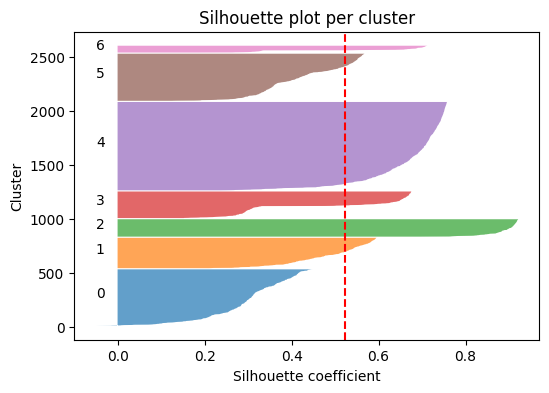
\includegraphics[keepaspectratio]{Notebooks/k7_files/figure-pdf/cell-15-output-1.png}}

\section{Feature Importance with
Classification}\label{feature-importance-with-classification}

\begin{Shaded}
\begin{Highlighting}[]
\NormalTok{t }\OperatorTok{=}\NormalTok{ DecisionTreeClassifier(max\_depth}\OperatorTok{=}\DecValTok{6}\NormalTok{, random\_state}\OperatorTok{=}\DecValTok{42}\NormalTok{)}
\NormalTok{feature\_cols }\OperatorTok{=}\NormalTok{ [col }\ControlFlowTok{for}\NormalTok{ col }\KeywordTok{in}\NormalTok{ df.columns }\ControlFlowTok{if}\NormalTok{ col }\OperatorTok{!=} \StringTok{"cluster\_abr"} \KeywordTok{and}\NormalTok{ col }\OperatorTok{!=} \StringTok{"cluster\_name"}\NormalTok{]}
\NormalTok{t.fit(df[feature\_cols], kmeans.labels\_)}
\NormalTok{feat\_imp }\OperatorTok{=}\NormalTok{ pd.Series(t.feature\_importances\_, index}\OperatorTok{=}\NormalTok{feature\_cols).sort\_values(ascending}\OperatorTok{=}\VariableTok{False}\NormalTok{)}
\NormalTok{feat\_imp}
\end{Highlighting}
\end{Shaded}

\begin{verbatim}
Surface Water Rights 2018-01-01    0.333920
cluster                            0.225944
PET 1996-11-01                     0.178228
Temp Min 2005-05-01                0.123259
Precipitation 1986-10-01           0.093196
                                     ...   
Temp Max 1987-08-01                0.000000
Temp Max 1987-07-01                0.000000
Temp Max 1987-06-01                0.000000
Temp Max 1987-05-01                0.000000
Temp Max 2019-10-01                0.000000
Length: 2291, dtype: float64
\end{verbatim}

Because of the way the data is formatted, interpret the above as general
groups of variables/times instead of specific dates. One specific column
or date might represent an overall trend. For example, surface water
rights in 2018 is not as important as the overall trend.

\begin{Shaded}
\begin{Highlighting}[]
\NormalTok{fig, ax }\OperatorTok{=}\NormalTok{ plt.subplots(figsize}\OperatorTok{=}\NormalTok{(}\DecValTok{18}\NormalTok{, }\DecValTok{10}\NormalTok{), dpi}\OperatorTok{=}\DecValTok{150}\NormalTok{)}
\NormalTok{tree.plot\_tree(}
\NormalTok{        t,}
\NormalTok{        feature\_names}\OperatorTok{=}\NormalTok{feature\_cols,}
\NormalTok{        class\_names}\OperatorTok{=}\NormalTok{[}\SpecialStringTok{f"C}\SpecialCharTok{\{}\NormalTok{i}\SpecialCharTok{\}}\SpecialStringTok{"} \ControlFlowTok{for}\NormalTok{ i }\KeywordTok{in} \BuiltInTok{sorted}\NormalTok{(}\BuiltInTok{set}\NormalTok{(df[}\StringTok{"cluster\_abr"}\NormalTok{]))],}
\NormalTok{        filled}\OperatorTok{=}\VariableTok{True}\NormalTok{,}
\NormalTok{        rounded}\OperatorTok{=}\VariableTok{True}\NormalTok{,}
\NormalTok{        fontsize}\OperatorTok{=}\DecValTok{8}\NormalTok{,}
\NormalTok{        ax}\OperatorTok{=}\NormalTok{ax)}
\NormalTok{plt.tight\_layout()}
\CommentTok{\# gini is a purity measurement, where gini=0 means this leaf contains all bofedales belonging to the cluster}
\end{Highlighting}
\end{Shaded}

\pandocbounded{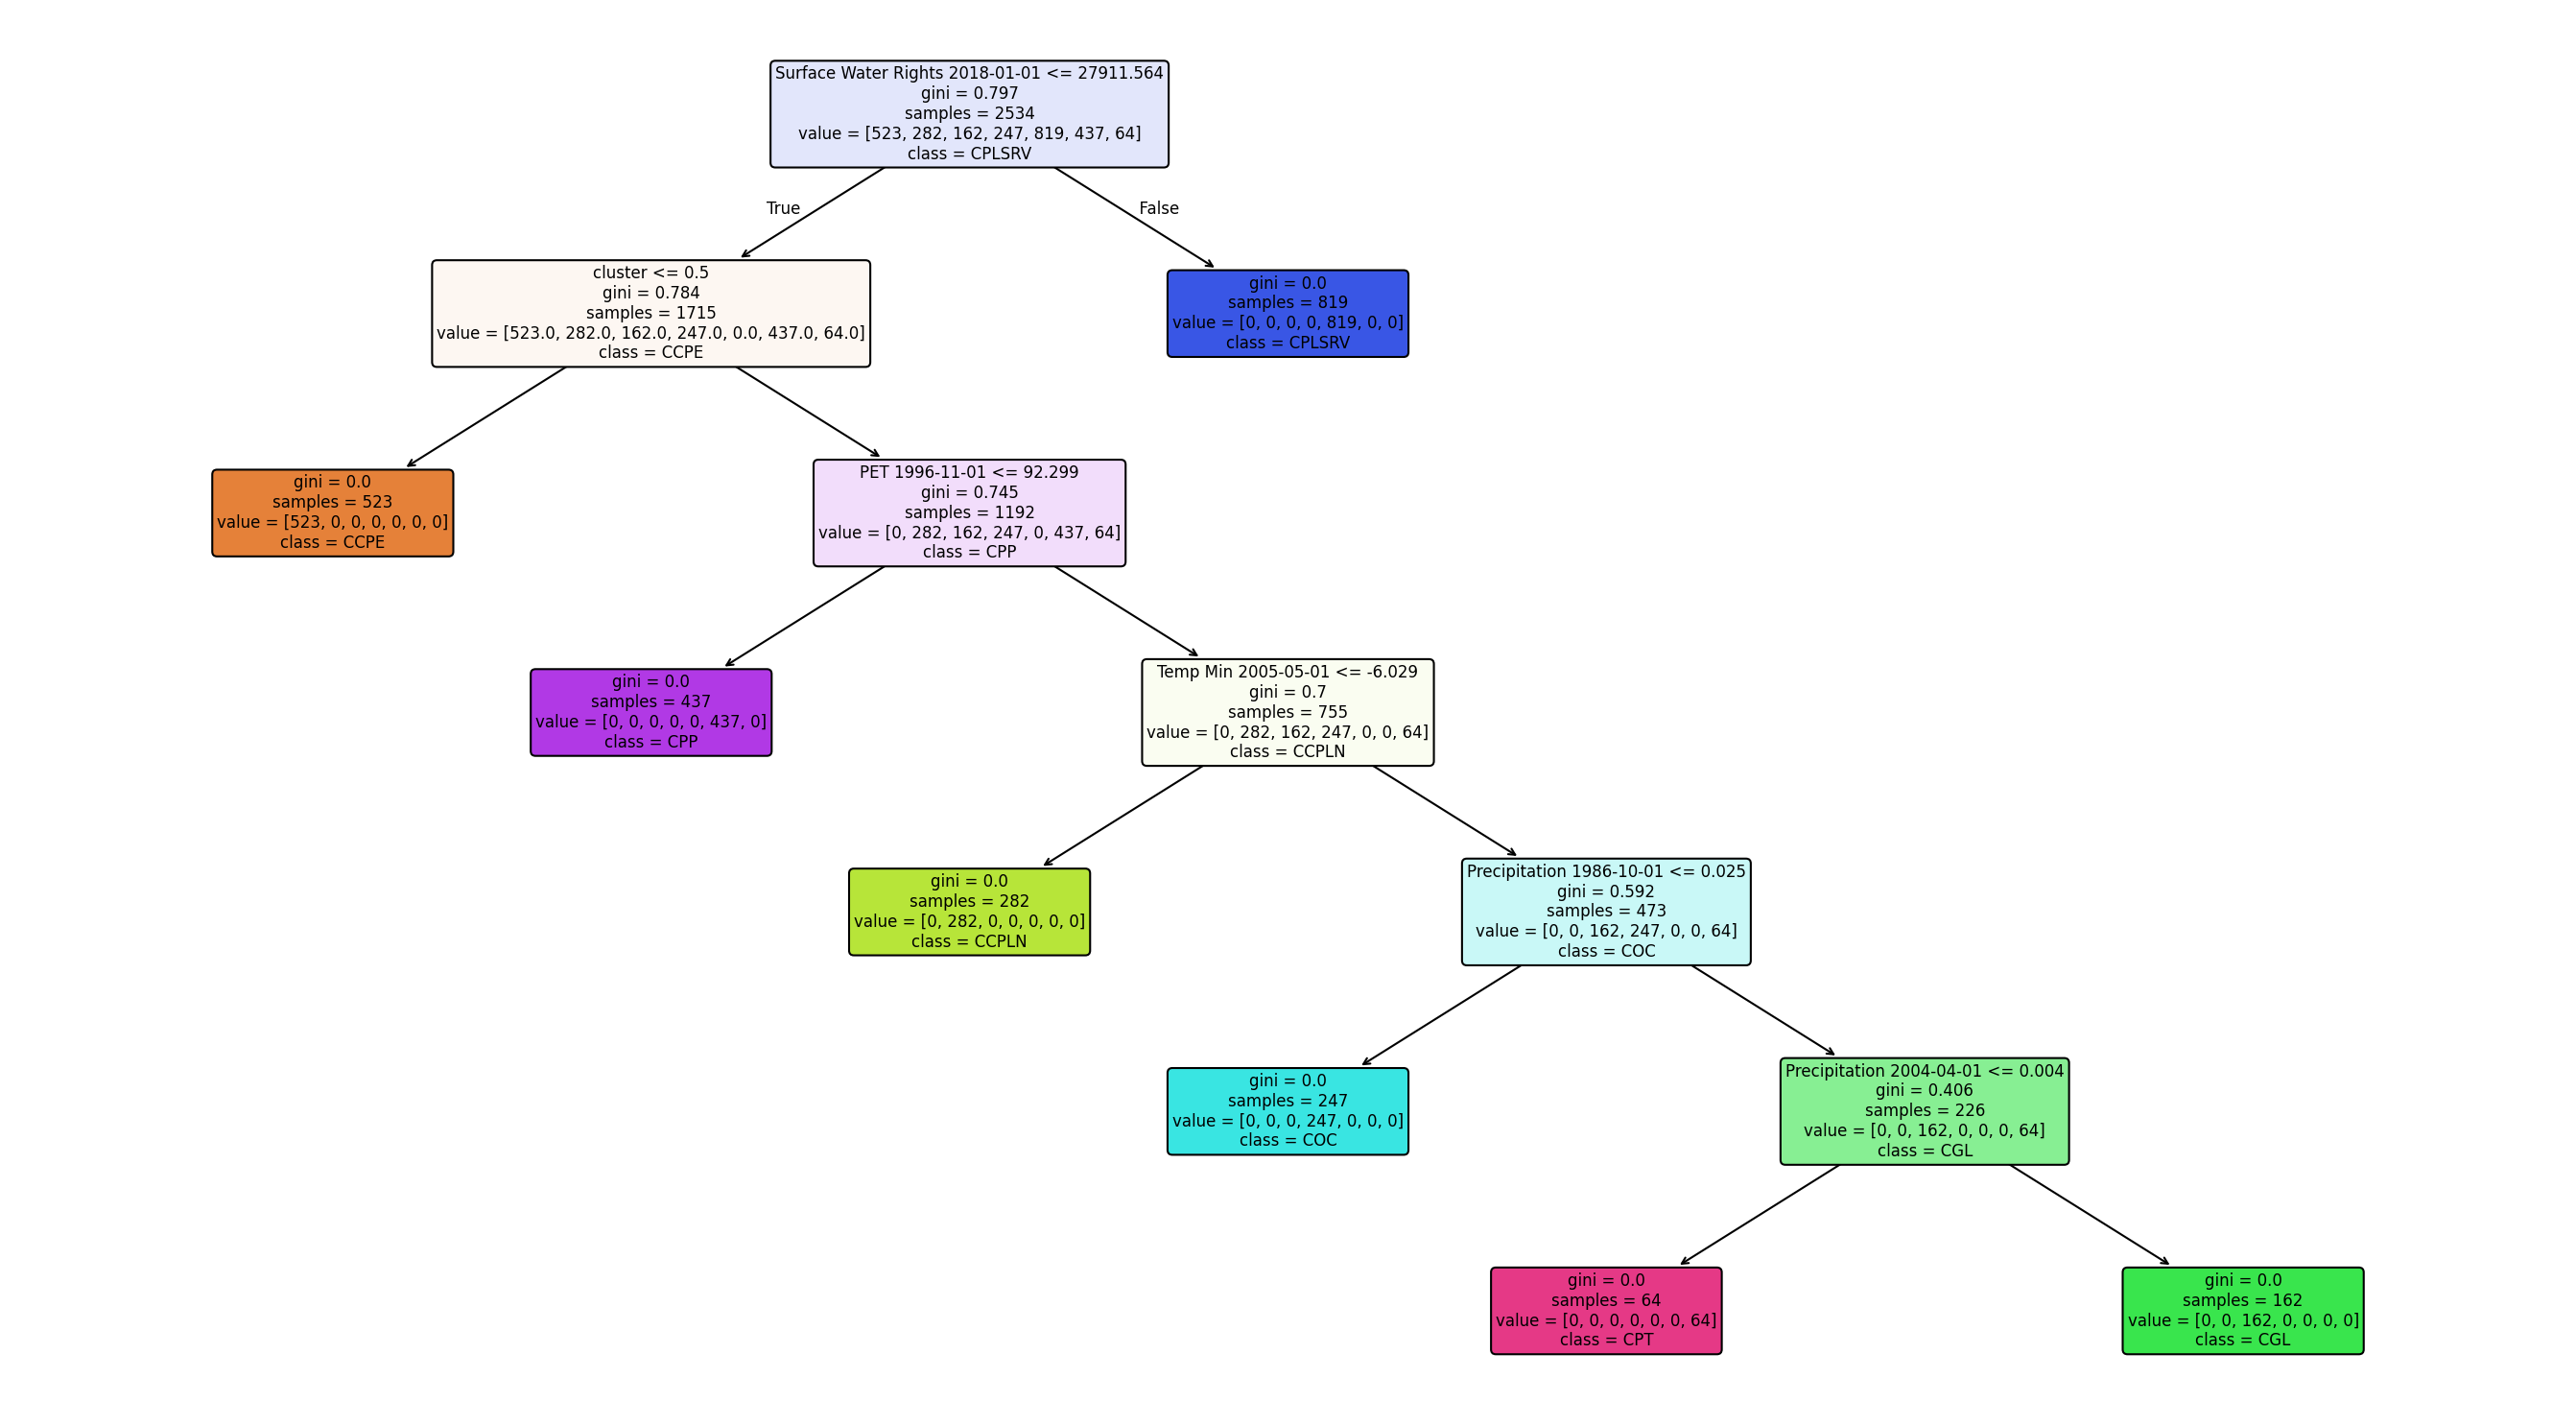
\includegraphics[keepaspectratio]{Notebooks/k7_files/figure-pdf/cell-17-output-1.png}}

\section{Data Visualizations}\label{data-visualizations}

\begin{Shaded}
\begin{Highlighting}[]
\NormalTok{pd.Series(df[}\StringTok{"cluster\_abr"}\NormalTok{]).value\_counts().sort\_index().plot.bar(color}\OperatorTok{=}\StringTok{\textquotesingle{}skyblue\textquotesingle{}}\NormalTok{)}
\NormalTok{plt.xlabel(}\StringTok{"Cluster"}\NormalTok{)}\OperatorTok{;}\NormalTok{ plt.ylabel(}\StringTok{"Count"}\NormalTok{)}
\NormalTok{plt.title(}\StringTok{"Number of bofedales per cluster"}\NormalTok{)}
\NormalTok{plt.xticks(rotation}\OperatorTok{=}\DecValTok{0}\NormalTok{)}
\NormalTok{plt.show()}
\end{Highlighting}
\end{Shaded}

\pandocbounded{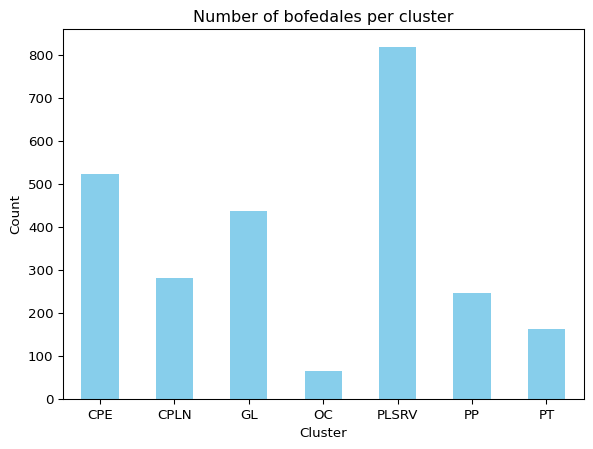
\includegraphics[keepaspectratio]{Notebooks/k7_files/figure-pdf/cell-18-output-1.png}}

\begin{Shaded}
\begin{Highlighting}[]
\NormalTok{geometry }\OperatorTok{=}\NormalTok{ [Point(xy) }\ControlFlowTok{for}\NormalTok{ xy }\KeywordTok{in} \BuiltInTok{zip}\NormalTok{(df.lon, df.lat)]}

\NormalTok{gdf }\OperatorTok{=}\NormalTok{ gpd.GeoDataFrame(}
\NormalTok{    df.copy(), }
\NormalTok{    geometry}\OperatorTok{=}\NormalTok{geometry,}
\NormalTok{    crs}\OperatorTok{=}\StringTok{"EPSG:4326"}
\NormalTok{)}

\NormalTok{gdf\_4326 }\OperatorTok{=}\NormalTok{ gdf.to\_crs(}\DecValTok{4326}\NormalTok{)}
\NormalTok{gdf\_4326[}\StringTok{"size\_for\_plot"}\NormalTok{] }\OperatorTok{=}\NormalTok{ gdf[}\StringTok{"Area\_m2"}\NormalTok{].}\BuiltInTok{apply}\NormalTok{(}\KeywordTok{lambda}\NormalTok{ a: (a}\OperatorTok{**}\FloatTok{0.5}\NormalTok{))}

\NormalTok{gdf\_4326[}\StringTok{"lon"}\NormalTok{] }\OperatorTok{=}\NormalTok{ gdf\_4326.geometry.x}
\NormalTok{gdf\_4326[}\StringTok{"lat"}\NormalTok{] }\OperatorTok{=}\NormalTok{ gdf\_4326.geometry.y}

\NormalTok{tab10 }\OperatorTok{=}\NormalTok{ plt.colormaps.get\_cmap(}\StringTok{"tab10"}\NormalTok{)}
\NormalTok{cluster\_ids }\OperatorTok{=} \BuiltInTok{sorted}\NormalTok{(gdf\_4326[}\StringTok{"cluster\_abr"}\NormalTok{].unique())}

\NormalTok{cluster\_colors }\OperatorTok{=}\NormalTok{ \{}
\NormalTok{    cid: mcolors.to\_hex(tab10(i }\OperatorTok{\%}\NormalTok{ tab10.N))}
    \ControlFlowTok{for}\NormalTok{ i, cid }\KeywordTok{in} \BuiltInTok{enumerate}\NormalTok{(cluster\_ids)}
\NormalTok{\}}

\NormalTok{center }\OperatorTok{=}\NormalTok{ [gdf\_4326.lat.mean(), gdf\_4326.lon.mean()]}
\NormalTok{m }\OperatorTok{=}\NormalTok{ folium.Map(center, zoom\_start}\OperatorTok{=}\DecValTok{6}\NormalTok{, tiles}\OperatorTok{=}\StringTok{"OpenStreetMap"}\NormalTok{)}

\NormalTok{sz }\OperatorTok{=}\NormalTok{ gdf\_4326[}\StringTok{"size\_for\_plot"}\NormalTok{]}
\NormalTok{radii }\OperatorTok{=}\NormalTok{ np.interp(sz, (sz.}\BuiltInTok{min}\NormalTok{(), sz.}\BuiltInTok{max}\NormalTok{()), (}\DecValTok{2}\NormalTok{, }\DecValTok{20}\NormalTok{))}

\ControlFlowTok{for}\NormalTok{ (\_, row), radius }\KeywordTok{in} \BuiltInTok{zip}\NormalTok{(gdf\_4326.iterrows(), radii):}
\NormalTok{    folium.CircleMarker(}
\NormalTok{        location}\OperatorTok{=}\NormalTok{(row.geometry.y, row.geometry.x),}
\NormalTok{        radius}\OperatorTok{=}\NormalTok{radius,}
\NormalTok{        fill}\OperatorTok{=}\VariableTok{True}\NormalTok{,}
\NormalTok{        fill\_opacity}\OperatorTok{=}\FloatTok{0.6}\NormalTok{,}
\NormalTok{        weight}\OperatorTok{=}\FloatTok{0.3}\NormalTok{,}
\NormalTok{        color}\OperatorTok{=}\StringTok{"black"}\NormalTok{,}
\NormalTok{        fill\_color}\OperatorTok{=}\NormalTok{cluster\_colors[row.cluster\_abr],}
\NormalTok{        popup}\OperatorTok{=}\NormalTok{(}
            \SpecialStringTok{f"Cluster }\SpecialCharTok{\{}\NormalTok{row}\SpecialCharTok{.}\NormalTok{cluster\_abr}\SpecialCharTok{\}}\SpecialStringTok{\textless{}br\textgreater{}"}
            \SpecialStringTok{f"Area = }\SpecialCharTok{\{}\NormalTok{row}\SpecialCharTok{.}\NormalTok{Area\_m2}\SpecialCharTok{:,\}}\SpecialStringTok{ m²"}
\NormalTok{        ),}
\NormalTok{    ).add\_to(m)}
\NormalTok{m}
\end{Highlighting}
\end{Shaded}

\begin{verbatim}
<folium.folium.Map at 0x15c05c680>
\end{verbatim}

\begin{Shaded}
\begin{Highlighting}[]
\NormalTok{unit\_mapping }\OperatorTok{=}\NormalTok{ \{}
    \StringTok{"Temp Min"}\NormalTok{: }\StringTok{"°C"}\NormalTok{, }
    \StringTok{"Temp Max"}\NormalTok{: }\StringTok{"°C"}\NormalTok{, }
    \StringTok{"Precipitation"}\NormalTok{: }\StringTok{"mm"}\NormalTok{, }
    \StringTok{"Ground Water Rights"}\NormalTok{: }\StringTok{"L/s"}\NormalTok{, }
    \StringTok{"Surface Water Rights"}\NormalTok{: }\StringTok{"L/s"}\NormalTok{, }
    \StringTok{"PET"}\NormalTok{: }\StringTok{"mm"}\NormalTok{, }
    \StringTok{"NDVI"}\NormalTok{: }\StringTok{""}\NormalTok{, }
    \StringTok{"NDWI"}\NormalTok{: }\StringTok{""}
\NormalTok{\}}
\NormalTok{vars\_order }\OperatorTok{=} \BuiltInTok{list}\NormalTok{(unit\_mapping.keys())}
\NormalTok{default\_var }\OperatorTok{=}\NormalTok{ vars\_order[}\DecValTok{0}\NormalTok{]}

\CommentTok{\# Optional guide{-}lines}
\NormalTok{guide\_lines }\OperatorTok{=}\NormalTok{ [}
    \CommentTok{\# \{"value": 0.0, "orientation": "h", "label": "Zero line", "color": "grey", "style": "dash", "width": 1\},}
\NormalTok{]}

\NormalTok{long\_parts }\OperatorTok{=}\NormalTok{ []}
\ControlFlowTok{for}\NormalTok{ var }\KeywordTok{in}\NormalTok{ vars\_order:}
\NormalTok{    var\_cols }\OperatorTok{=}\NormalTok{ [c }\ControlFlowTok{for}\NormalTok{ c }\KeywordTok{in}\NormalTok{ df.columns }\ControlFlowTok{if}\NormalTok{ c.startswith(}\SpecialStringTok{f"}\SpecialCharTok{\{}\NormalTok{var}\SpecialCharTok{\}}\SpecialStringTok{ "}\NormalTok{)]}
    \ControlFlowTok{if} \KeywordTok{not}\NormalTok{ var\_cols:}
        \ControlFlowTok{continue}

\NormalTok{    block }\OperatorTok{=}\NormalTok{ df[var\_cols }\OperatorTok{+}\NormalTok{ [}\StringTok{"cluster\_abr"}\NormalTok{]].copy()}
\NormalTok{    date\_index }\OperatorTok{=}\NormalTok{ pd.to\_datetime(}
\NormalTok{        [c.replace(}\SpecialStringTok{f"}\SpecialCharTok{\{}\NormalTok{var}\SpecialCharTok{\}}\SpecialStringTok{ "}\NormalTok{, }\StringTok{""}\NormalTok{) }\ControlFlowTok{for}\NormalTok{ c }\KeywordTok{in}\NormalTok{ var\_cols], errors}\OperatorTok{=}\StringTok{"raise"}
\NormalTok{    )}
\NormalTok{    block.columns }\OperatorTok{=}\NormalTok{ date\_index.tolist() }\OperatorTok{+}\NormalTok{ [}\StringTok{"cluster\_abr"}\NormalTok{]}

\NormalTok{    block }\OperatorTok{=}\NormalTok{ block.melt(id\_vars}\OperatorTok{=}\StringTok{"cluster\_abr"}\NormalTok{, var\_name}\OperatorTok{=}\StringTok{"date"}\NormalTok{, value\_name}\OperatorTok{=}\StringTok{"value"}\NormalTok{)}
\NormalTok{    block[}\StringTok{"variable"}\NormalTok{] }\OperatorTok{=}\NormalTok{ var}
\NormalTok{    block[}\StringTok{"date"}\NormalTok{] }\OperatorTok{=}\NormalTok{ pd.to\_datetime(block[}\StringTok{"date"}\NormalTok{], errors}\OperatorTok{=}\StringTok{"raise"}\NormalTok{)}

\NormalTok{    long\_parts.append(block)}

\NormalTok{tidy }\OperatorTok{=}\NormalTok{ pd.concat(long\_parts, ignore\_index}\OperatorTok{=}\VariableTok{True}\NormalTok{)}

\NormalTok{tidy[}\StringTok{"year"}\NormalTok{] }\OperatorTok{=}\NormalTok{ tidy[}\StringTok{"date"}\NormalTok{].dt.year}
\NormalTok{tidy\_annual }\OperatorTok{=}\NormalTok{ (}
\NormalTok{    tidy}
\NormalTok{      .groupby([}\StringTok{"cluster\_abr"}\NormalTok{, }\StringTok{"variable"}\NormalTok{, }\StringTok{"year"}\NormalTok{], as\_index}\OperatorTok{=}\VariableTok{False}\NormalTok{)}
\NormalTok{      .mean(numeric\_only}\OperatorTok{=}\VariableTok{True}\NormalTok{)}
\NormalTok{)}

\NormalTok{clusters }\OperatorTok{=}\NormalTok{ tidy\_annual[}\StringTok{"cluster\_abr"}\NormalTok{].unique()}

\NormalTok{fig }\OperatorTok{=}\NormalTok{ go.Figure()}

\ControlFlowTok{for}\NormalTok{ clus }\KeywordTok{in}\NormalTok{ clusters:}
\NormalTok{    sub }\OperatorTok{=}\NormalTok{ tidy\_annual.query(}\StringTok{"cluster\_abr == @clus and variable == @default\_var"}\NormalTok{)}
\NormalTok{    fig.add\_trace(}
\NormalTok{        go.Scatter(}
\NormalTok{            x}\OperatorTok{=}\NormalTok{sub[}\StringTok{"year"}\NormalTok{],}
\NormalTok{            y}\OperatorTok{=}\NormalTok{sub[}\StringTok{"value"}\NormalTok{],}
\NormalTok{            mode}\OperatorTok{=}\StringTok{"lines"}\NormalTok{,}
\NormalTok{            name}\OperatorTok{=}\NormalTok{clus,}
\NormalTok{            line}\OperatorTok{=}\BuiltInTok{dict}\NormalTok{(color}\OperatorTok{=}\NormalTok{cluster\_palette[clus], width}\OperatorTok{=}\DecValTok{2}\NormalTok{)}
\NormalTok{        )}
\NormalTok{    )}

\ControlFlowTok{for}\NormalTok{ ln }\KeywordTok{in}\NormalTok{ guide\_lines:}
    \ControlFlowTok{if}\NormalTok{ ln[}\StringTok{"orientation"}\NormalTok{].lower().startswith(}\StringTok{"h"}\NormalTok{):}
\NormalTok{        fig.add\_shape(}
            \BuiltInTok{type}\OperatorTok{=}\StringTok{"line"}\NormalTok{,}
\NormalTok{            x0}\OperatorTok{=}\NormalTok{tidy\_annual[}\StringTok{"year"}\NormalTok{].}\BuiltInTok{min}\NormalTok{(), x1}\OperatorTok{=}\NormalTok{tidy\_annual[}\StringTok{"year"}\NormalTok{].}\BuiltInTok{max}\NormalTok{(),}
\NormalTok{            y0}\OperatorTok{=}\NormalTok{ln[}\StringTok{"value"}\NormalTok{], y1}\OperatorTok{=}\NormalTok{ln[}\StringTok{"value"}\NormalTok{],}
\NormalTok{            line}\OperatorTok{=}\BuiltInTok{dict}\NormalTok{(color}\OperatorTok{=}\NormalTok{ln.get(}\StringTok{"color"}\NormalTok{, }\StringTok{"red"}\NormalTok{),}
\NormalTok{                      dash}\OperatorTok{=}\NormalTok{ln.get(}\StringTok{"style"}\NormalTok{, }\StringTok{"dash"}\NormalTok{),}
\NormalTok{                      width}\OperatorTok{=}\NormalTok{ln.get(}\StringTok{"width"}\NormalTok{, }\DecValTok{2}\NormalTok{))}
\NormalTok{        )}
    \ControlFlowTok{else}\NormalTok{:}
\NormalTok{        fig.add\_shape(}
            \BuiltInTok{type}\OperatorTok{=}\StringTok{"line"}\NormalTok{,}
\NormalTok{            y0}\OperatorTok{=}\NormalTok{tidy\_annual[}\StringTok{"value"}\NormalTok{].}\BuiltInTok{min}\NormalTok{(), y1}\OperatorTok{=}\NormalTok{tidy\_annual[}\StringTok{"value"}\NormalTok{].}\BuiltInTok{max}\NormalTok{(),}
\NormalTok{            x0}\OperatorTok{=}\NormalTok{ln[}\StringTok{"value"}\NormalTok{], x1}\OperatorTok{=}\NormalTok{ln[}\StringTok{"value"}\NormalTok{],}
\NormalTok{            line}\OperatorTok{=}\BuiltInTok{dict}\NormalTok{(color}\OperatorTok{=}\NormalTok{ln.get(}\StringTok{"color"}\NormalTok{, }\StringTok{"red"}\NormalTok{),}
\NormalTok{                      dash}\OperatorTok{=}\NormalTok{ln.get(}\StringTok{"style"}\NormalTok{, }\StringTok{"dash"}\NormalTok{),}
\NormalTok{                      width}\OperatorTok{=}\NormalTok{ln.get(}\StringTok{"width"}\NormalTok{, }\DecValTok{2}\NormalTok{))}
\NormalTok{        )}

\NormalTok{buttons }\OperatorTok{=}\NormalTok{ []}
\ControlFlowTok{for}\NormalTok{ var }\KeywordTok{in}\NormalTok{ vars\_order:}
\NormalTok{    ys }\OperatorTok{=}\NormalTok{ [}
\NormalTok{        tidy\_annual.query(}\StringTok{"cluster\_abr == @clus and variable == @var"}\NormalTok{)[}\StringTok{"value"}\NormalTok{].values}
        \ControlFlowTok{for}\NormalTok{ clus }\KeywordTok{in}\NormalTok{ clusters}
\NormalTok{    ]}
\NormalTok{    label }\OperatorTok{=}\NormalTok{ var }\OperatorTok{+}\NormalTok{ (}\SpecialStringTok{f" (}\SpecialCharTok{\{}\NormalTok{unit\_mapping[var]}\SpecialCharTok{\}}\SpecialStringTok{)"} \ControlFlowTok{if}\NormalTok{ unit\_mapping[var] }\ControlFlowTok{else} \StringTok{""}\NormalTok{)}
\NormalTok{    buttons.append(}
        \BuiltInTok{dict}\NormalTok{(}
\NormalTok{            label  }\OperatorTok{=}\NormalTok{ var,}
\NormalTok{            method }\OperatorTok{=} \StringTok{"update"}\NormalTok{,}
\NormalTok{            args   }\OperatorTok{=}\NormalTok{ [}
\NormalTok{                \{}\StringTok{"y"}\NormalTok{: ys\},}
\NormalTok{                \{}
                  \StringTok{"title"}\NormalTok{: }\SpecialStringTok{f"Average }\SpecialCharTok{\{}\NormalTok{var}\SpecialCharTok{\}}\SpecialStringTok{ by Cluster"}\NormalTok{,}
                  \StringTok{"yaxis"}\NormalTok{: \{}\StringTok{"title"}\NormalTok{: \{}\StringTok{"text"}\NormalTok{: label\}\}}
\NormalTok{                \}}
\NormalTok{            ]}
\NormalTok{        )}
\NormalTok{    )}

\NormalTok{fig.update\_layout(}
\NormalTok{    xaxis\_title}\OperatorTok{=}\StringTok{"Year"}\NormalTok{,}
\NormalTok{    yaxis\_title}\OperatorTok{=}\SpecialStringTok{f"}\SpecialCharTok{\{}\NormalTok{default\_var}\SpecialCharTok{\}}\SpecialStringTok{"} \OperatorTok{+}\NormalTok{ (}\SpecialStringTok{f" (}\SpecialCharTok{\{}\NormalTok{unit\_mapping[default\_var]}\SpecialCharTok{\}}\SpecialStringTok{)"} \ControlFlowTok{if}\NormalTok{ unit\_mapping[default\_var] }\ControlFlowTok{else} \StringTok{""}\NormalTok{),}
\NormalTok{    updatemenus}\OperatorTok{=}\NormalTok{[}\BuiltInTok{dict}\NormalTok{(}
        \BuiltInTok{type}\OperatorTok{=}\StringTok{"dropdown"}\NormalTok{,}
\NormalTok{        direction}\OperatorTok{=}\StringTok{"down"}\NormalTok{,}
\NormalTok{        showactive}\OperatorTok{=}\VariableTok{True}\NormalTok{,}
\NormalTok{        buttons}\OperatorTok{=}\NormalTok{buttons,}
\NormalTok{        x}\OperatorTok{=}\FloatTok{0.0}\NormalTok{, xanchor}\OperatorTok{=}\StringTok{"left"}\NormalTok{,}
\NormalTok{        y}\OperatorTok{=}\FloatTok{1.15}\NormalTok{, yanchor}\OperatorTok{=}\StringTok{"top"}
\NormalTok{    )],}
\NormalTok{    legend\_title\_text}\OperatorTok{=}\StringTok{"Cluster"}\NormalTok{,}
\NormalTok{    height}\OperatorTok{=}\DecValTok{500}\NormalTok{, width}\OperatorTok{=}\DecValTok{900}\NormalTok{,}
\NormalTok{    margin}\OperatorTok{=}\BuiltInTok{dict}\NormalTok{(t}\OperatorTok{=}\DecValTok{90}\NormalTok{, r}\OperatorTok{=}\DecValTok{20}\NormalTok{, l}\OperatorTok{=}\DecValTok{60}\NormalTok{, b}\OperatorTok{=}\DecValTok{50}\NormalTok{)}
\NormalTok{)}

\NormalTok{fig}
\end{Highlighting}
\end{Shaded}

\begin{verbatim}
Unable to display output for mime type(s): text/html
\end{verbatim}

\begin{verbatim}
Unable to display output for mime type(s): text/html
\end{verbatim}

\begin{Shaded}
\begin{Highlighting}[]
\NormalTok{palette }\OperatorTok{=}\NormalTok{ [}
    \StringTok{"indianred"}\NormalTok{,}\StringTok{"lightsalmon"}\NormalTok{,}\StringTok{"mediumaquamarine"}\NormalTok{,}\StringTok{"powderblue"}\NormalTok{,}\StringTok{"darkslateblue"}\NormalTok{,}
    \StringTok{"mediumturquoise"}\NormalTok{,}\StringTok{"lavender"}\NormalTok{,}\StringTok{"palevioletred"}\NormalTok{,}\StringTok{"olivedrab"}\NormalTok{,}\StringTok{"lightpink"}\NormalTok{,}
    \StringTok{"gold"}\NormalTok{,}\StringTok{"mediumvioletred"}\NormalTok{,}\StringTok{"lightcoral"}\NormalTok{,}\StringTok{"tomato"}\NormalTok{,}\StringTok{"sandybrown"}\NormalTok{,}
\NormalTok{]}

\NormalTok{df\_condensed }\OperatorTok{=}\NormalTok{ (}
\NormalTok{    df[[}\StringTok{\textquotesingle{}Area\_m2\textquotesingle{}}\NormalTok{, }\StringTok{\textquotesingle{}AUC\textquotesingle{}}\NormalTok{, }\StringTok{\textquotesingle{}pct\_prot\textquotesingle{}}\NormalTok{, }\StringTok{\textquotesingle{}elev\_mean\_\textquotesingle{}}\NormalTok{, }\StringTok{\textquotesingle{}elev\_std\_m\textquotesingle{}}\NormalTok{,}
        \StringTok{\textquotesingle{}n\_wells\textquotesingle{}}\NormalTok{, }\StringTok{\textquotesingle{}cluster\textquotesingle{}}\NormalTok{, }\StringTok{\textquotesingle{}cluster\_abr\textquotesingle{}}\NormalTok{]]}
\NormalTok{      .rename(columns}\OperatorTok{=}\NormalTok{\{}
          \StringTok{\textquotesingle{}pct\_prot\textquotesingle{}}\NormalTok{: }\StringTok{\textquotesingle{}Percentage Protected Land (of total bofedal)\textquotesingle{}}\NormalTok{,}
          \StringTok{\textquotesingle{}Area\_m2\textquotesingle{}}\NormalTok{ : }\StringTok{\textquotesingle{}Area (in m²)\textquotesingle{}}\NormalTok{,}
          \StringTok{\textquotesingle{}AUC\textquotesingle{}}\NormalTok{     : }\StringTok{\textquotesingle{}Area of basin\textquotesingle{}}\NormalTok{,}
          \StringTok{\textquotesingle{}elev\_mean\_\textquotesingle{}}\NormalTok{: }\StringTok{\textquotesingle{}Average Elevation (in m)\textquotesingle{}}\NormalTok{,}
          \StringTok{\textquotesingle{}elev\_std\_m\textquotesingle{}}\NormalTok{: }\StringTok{\textquotesingle{}Elevation Standard Deviation (in m)\textquotesingle{}}\NormalTok{,}
          \StringTok{\textquotesingle{}n\_wells\textquotesingle{}}\NormalTok{   : }\StringTok{\textquotesingle{}Number of wells (per catchment area)\textquotesingle{}}\NormalTok{,}
\NormalTok{      \})}
\NormalTok{)}

\NormalTok{agg }\OperatorTok{=}\NormalTok{ (df\_condensed}
\NormalTok{       .groupby(}\StringTok{"cluster\_abr"}\NormalTok{, as\_index}\OperatorTok{=}\VariableTok{False}\NormalTok{)}
\NormalTok{       .mean())}

\KeywordTok{def}\NormalTok{ make\_trace(var, colour):}
    \ControlFlowTok{return}\NormalTok{ go.Bar(}
\NormalTok{        x}\OperatorTok{=}\NormalTok{agg[}\StringTok{"cluster\_abr"}\NormalTok{],}
\NormalTok{        y}\OperatorTok{=}\NormalTok{agg[var],}
\NormalTok{        marker}\OperatorTok{=}\BuiltInTok{dict}\NormalTok{(color}\OperatorTok{=}\NormalTok{colour, line}\OperatorTok{=}\BuiltInTok{dict}\NormalTok{(color}\OperatorTok{=}\StringTok{"black"}\NormalTok{)),}
\NormalTok{        name}\OperatorTok{=}\NormalTok{var}
\NormalTok{    )}

\NormalTok{vars\_list   }\OperatorTok{=} \BuiltInTok{list}\NormalTok{(agg.columns[}\DecValTok{1}\NormalTok{:])}
\NormalTok{default\_var }\OperatorTok{=}\NormalTok{ vars\_list[}\DecValTok{0}\NormalTok{]}

\NormalTok{fig }\OperatorTok{=}\NormalTok{ go.Figure(make\_trace(default\_var, palette[}\DecValTok{0}\NormalTok{]))}

\NormalTok{buttons }\OperatorTok{=}\NormalTok{ []}
\ControlFlowTok{for}\NormalTok{ i, var }\KeywordTok{in} \BuiltInTok{enumerate}\NormalTok{(vars\_list):}
\NormalTok{    buttons.append(}
        \BuiltInTok{dict}\NormalTok{(}
\NormalTok{            label  }\OperatorTok{=}\NormalTok{ var,}
\NormalTok{            method }\OperatorTok{=} \StringTok{"update"}\NormalTok{,}
\NormalTok{            args   }\OperatorTok{=}\NormalTok{ [}
\NormalTok{                \{}\StringTok{"y"}\NormalTok{: [agg[var]],}
                 \StringTok{"marker.color"}\NormalTok{: [palette[i }\OperatorTok{\%} \BuiltInTok{len}\NormalTok{(palette)]]\},}
\NormalTok{                \{}
                  \StringTok{"yaxis"}\NormalTok{: \{}\StringTok{"title"}\NormalTok{: \{}\StringTok{"text"}\NormalTok{: var\}\}}
\NormalTok{                \}}
\NormalTok{            ]}
\NormalTok{        )}
\NormalTok{    )}

\NormalTok{fig.update\_layout(}
\NormalTok{    title}\OperatorTok{=}\StringTok{""}\NormalTok{,}
\NormalTok{    yaxis}\OperatorTok{=}\BuiltInTok{dict}\NormalTok{(title}\OperatorTok{=}\BuiltInTok{dict}\NormalTok{(text}\OperatorTok{=}\NormalTok{default\_var)),}
\NormalTok{    xaxis}\OperatorTok{=}\BuiltInTok{dict}\NormalTok{(}
\NormalTok{        title}\OperatorTok{=}\StringTok{"Cluster"}\NormalTok{,}
        \BuiltInTok{type}\OperatorTok{=}\StringTok{"category"}\NormalTok{,}
\NormalTok{        categoryorder}\OperatorTok{=}\StringTok{"array"}\NormalTok{,}
\NormalTok{        categoryarray}\OperatorTok{=}\NormalTok{agg[}\StringTok{"cluster\_abr"}\NormalTok{].tolist()}
\NormalTok{    ),}
\NormalTok{    updatemenus}\OperatorTok{=}\NormalTok{[}\BuiltInTok{dict}\NormalTok{(}
        \BuiltInTok{type}\OperatorTok{=}\StringTok{"dropdown"}\NormalTok{,}
\NormalTok{        direction}\OperatorTok{=}\StringTok{"down"}\NormalTok{,}
\NormalTok{        showactive}\OperatorTok{=}\VariableTok{True}\NormalTok{,}
\NormalTok{        buttons}\OperatorTok{=}\NormalTok{buttons,}
\NormalTok{        x}\OperatorTok{=}\FloatTok{0.0}\NormalTok{, xanchor}\OperatorTok{=}\StringTok{"left"}\NormalTok{,}
\NormalTok{        y}\OperatorTok{=}\FloatTok{1.15}\NormalTok{, yanchor}\OperatorTok{=}\StringTok{"top"}
\NormalTok{    )],}
\NormalTok{    margin}\OperatorTok{=}\BuiltInTok{dict}\NormalTok{(t}\OperatorTok{=}\DecValTok{60}\NormalTok{, r}\OperatorTok{=}\DecValTok{20}\NormalTok{, l}\OperatorTok{=}\DecValTok{60}\NormalTok{, b}\OperatorTok{=}\DecValTok{50}\NormalTok{),}
\NormalTok{    height}\OperatorTok{=}\DecValTok{450}\NormalTok{, width}\OperatorTok{=}\DecValTok{700}\NormalTok{,}
\NormalTok{    showlegend}\OperatorTok{=}\VariableTok{False}
\NormalTok{)}


\NormalTok{fig}
\end{Highlighting}
\end{Shaded}

\begin{verbatim}
Unable to display output for mime type(s): text/html
\end{verbatim}

\chapter{Running k=2}\label{running-k2}

\section{Loading the data and importing
packages}\label{loading-the-data-and-importing-packages}

\begin{Shaded}
\begin{Highlighting}[]
\ImportTok{from}\NormalTok{ sklearn.preprocessing }\ImportTok{import}\NormalTok{ StandardScaler}
\ImportTok{from}\NormalTok{ sklearn.decomposition }\ImportTok{import}\NormalTok{ PCA}
\ImportTok{from}\NormalTok{ sklearn.cluster }\ImportTok{import}\NormalTok{ KMeans}
\ImportTok{from}\NormalTok{ sklearn.metrics }\ImportTok{import}\NormalTok{ silhouette\_score, calinski\_harabasz\_score, davies\_bouldin\_score, pairwise\_distances\_argmin\_min, silhouette\_samples}

\ImportTok{import}\NormalTok{ pandas }\ImportTok{as}\NormalTok{ pd}
\ImportTok{import}\NormalTok{ numpy }\ImportTok{as}\NormalTok{ np}
\ImportTok{import}\NormalTok{ matplotlib.pyplot }\ImportTok{as}\NormalTok{ plt}

\ImportTok{import}\NormalTok{ geopandas }\ImportTok{as}\NormalTok{ gpd}
\ImportTok{from}\NormalTok{ shapely.geometry }\ImportTok{import}\NormalTok{ Point}
\ImportTok{import}\NormalTok{ contextily }\ImportTok{as}\NormalTok{ ctx}
\ImportTok{from}\NormalTok{ matplotlib.lines }\ImportTok{import}\NormalTok{ Line2D}
\ImportTok{import}\NormalTok{ matplotlib.dates }\ImportTok{as}\NormalTok{ mdates}
\ImportTok{import}\NormalTok{ matplotlib.colors }\ImportTok{as}\NormalTok{ mcolors}
\ImportTok{import}\NormalTok{ matplotlib.cm }\ImportTok{as}\NormalTok{ cm}
\ImportTok{import}\NormalTok{ folium}
\end{Highlighting}
\end{Shaded}

\begin{Shaded}
\begin{Highlighting}[]
\NormalTok{X\_ }\OperatorTok{=}\NormalTok{ np.load(}\StringTok{"scaled{-}df.npy"}\NormalTok{)}
\NormalTok{df }\OperatorTok{=}\NormalTok{ pd.read\_csv(}\StringTok{"bofedales{-}clean.csv"}\NormalTok{)}
\NormalTok{df.drop(}\StringTok{"Unnamed: 0"}\NormalTok{, axis}\OperatorTok{=}\DecValTok{1}\NormalTok{, inplace}\OperatorTok{=}\VariableTok{True}\NormalTok{)}
\NormalTok{df.head(}\DecValTok{1}\NormalTok{)}
\end{Highlighting}
\end{Shaded}

\begin{longtable}[]{@{}llllllllllllllllllllll@{}}
\toprule\noalign{}
& Area\_m2 & AUC & pct\_prot & elev\_mean\_ & elev\_std\_m & n\_wells &
Ground Water Rights 1966-01-01 & Ground Water Rights 1967-01-01 & Ground
Water Rights 1968-01-01 & Ground Water Rights 1969-01-01 & ... & NDWI
2019-03 & NDWI 2019-04 & NDWI 2019-05 & NDWI 2019-06 & NDWI 2019-07 &
NDWI 2019-08 & NDWI 2019-09 & NDWI 2019-10 & NDWI 2019-11 & NDWI
2019-12 \\
\midrule\noalign{}
\endhead
\bottomrule\noalign{}
\endlastfoot
0 & 6300 & 86.769539 & 0.0 & 4162.714286 & 3.953815 & 0.0 & 0.0 & 0.0 &
0.0 & 0.0 & ... & 0.03193 & 0.026136 & 0.022087 & 0.019181 & 0.023405 &
0.015355 & -0.000504 & 0.004056 & 0.014678 & 0.010436 \\
\end{longtable}

\section{Running k=2}\label{running-k2-1}

\begin{Shaded}
\begin{Highlighting}[]
\NormalTok{K}\OperatorTok{=}\DecValTok{2}
\NormalTok{kmeans }\OperatorTok{=}\NormalTok{ KMeans(n\_clusters}\OperatorTok{=}\NormalTok{K, random\_state}\OperatorTok{=}\DecValTok{42}\NormalTok{, n\_init}\OperatorTok{=}\DecValTok{20}\NormalTok{)}
\NormalTok{cluster\_labels }\OperatorTok{=}\NormalTok{ kmeans.fit\_predict(X\_)}
\NormalTok{centroids\_pca }\OperatorTok{=}\NormalTok{ kmeans.cluster\_centers\_ }
\end{Highlighting}
\end{Shaded}

\begin{Shaded}
\begin{Highlighting}[]
\NormalTok{df[}\StringTok{"cluster"}\NormalTok{] }\OperatorTok{=}\NormalTok{ cluster\_labels}
\end{Highlighting}
\end{Shaded}

\subsection{Measuring fit}\label{measuring-fit}

\begin{Shaded}
\begin{Highlighting}[]
\NormalTok{inertia }\OperatorTok{=}\NormalTok{ kmeans.inertia\_}

\NormalTok{avg\_sq\_dist\_per\_sample }\OperatorTok{=}\NormalTok{ inertia }\OperatorTok{/}\NormalTok{ X\_.shape[}\DecValTok{0}\NormalTok{]}

\BuiltInTok{print}\NormalTok{(}\SpecialStringTok{f"Average squared distance per point: }\SpecialCharTok{\{}\NormalTok{avg\_sq\_dist\_per\_sample}\SpecialCharTok{:.4f\}}\SpecialStringTok{"}\NormalTok{)}

\NormalTok{mu }\OperatorTok{=}\NormalTok{ X\_.mean(axis}\OperatorTok{=}\DecValTok{0}\NormalTok{)}
\NormalTok{global\_mse }\OperatorTok{=}\NormalTok{ ((X\_ }\OperatorTok{{-}}\NormalTok{ mu)}\OperatorTok{**}\DecValTok{2}\NormalTok{).}\BuiltInTok{sum}\NormalTok{(axis}\OperatorTok{=}\DecValTok{1}\NormalTok{).mean()}
\BuiltInTok{print}\NormalTok{(}\SpecialStringTok{f"Global mean: }\SpecialCharTok{\{}\NormalTok{global\_mse}\SpecialCharTok{\}}\SpecialStringTok{"}\NormalTok{)}
\end{Highlighting}
\end{Shaded}

\begin{verbatim}
Average squared distance per point: 907.8377
Global mean: 2159.8318653940732
\end{verbatim}

\begin{Shaded}
\begin{Highlighting}[]
\NormalTok{pca2 }\OperatorTok{=}\NormalTok{ PCA(n\_components}\OperatorTok{=}\DecValTok{2}\NormalTok{).fit\_transform(X\_)}
\NormalTok{plt.scatter(pca2[:,}\DecValTok{0}\NormalTok{], pca2[:,}\DecValTok{1}\NormalTok{], c}\OperatorTok{=}\NormalTok{cluster\_labels, s}\OperatorTok{=}\DecValTok{10}\NormalTok{, cmap}\OperatorTok{=}\StringTok{\textquotesingle{}plasma\textquotesingle{}}\NormalTok{)}
\NormalTok{plt.xlabel(}\StringTok{\textquotesingle{}PC1\textquotesingle{}}\NormalTok{)}\OperatorTok{;}\NormalTok{ plt.ylabel(}\StringTok{\textquotesingle{}PC2\textquotesingle{}}\NormalTok{)}
\NormalTok{plt.title(}\StringTok{\textquotesingle{}K{-}means clusters in PCA space\textquotesingle{}}\NormalTok{)}
\NormalTok{plt.colorbar()}
\NormalTok{plt.show()}
\end{Highlighting}
\end{Shaded}

\pandocbounded{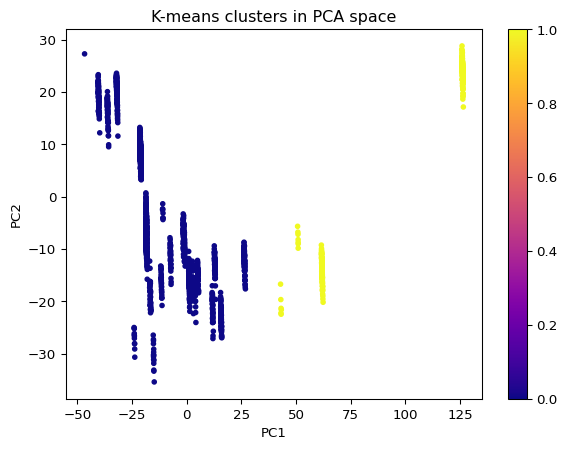
\includegraphics[keepaspectratio]{Notebooks/k2_files/figure-pdf/cell-7-output-1.png}}

\section{Data Visualizations}\label{data-visualizations-1}

\begin{Shaded}
\begin{Highlighting}[]
\NormalTok{pd.Series(df[}\StringTok{"cluster"}\NormalTok{]).value\_counts().sort\_index().plot.bar(color}\OperatorTok{=}\StringTok{\textquotesingle{}skyblue\textquotesingle{}}\NormalTok{)}
\NormalTok{plt.xlabel(}\StringTok{"Cluster"}\NormalTok{)}\OperatorTok{;}\NormalTok{ plt.ylabel(}\StringTok{"Count"}\NormalTok{)}
\NormalTok{plt.title(}\StringTok{"Number of bofedales per cluster"}\NormalTok{)}
\NormalTok{plt.xticks(rotation}\OperatorTok{=}\DecValTok{0}\NormalTok{)}
\NormalTok{plt.show()}
\end{Highlighting}
\end{Shaded}

\pandocbounded{\includegraphics[keepaspectratio]{Notebooks/k2_files/figure-pdf/cell-8-output-1.png}}

\begin{Shaded}
\begin{Highlighting}[]
\NormalTok{geometry }\OperatorTok{=}\NormalTok{ [Point(xy) }\ControlFlowTok{for}\NormalTok{ xy }\KeywordTok{in} \BuiltInTok{zip}\NormalTok{(df.lon, df.lat)]}

\NormalTok{gdf }\OperatorTok{=}\NormalTok{ gpd.GeoDataFrame(}
\NormalTok{    df.copy(), }
\NormalTok{    geometry}\OperatorTok{=}\NormalTok{geometry,}
\NormalTok{    crs}\OperatorTok{=}\StringTok{"EPSG:4326"}
\NormalTok{)}

\NormalTok{gdf[}\StringTok{"size\_for\_plot"}\NormalTok{] }\OperatorTok{=}\NormalTok{ gdf[}\StringTok{"Area\_m2"}\NormalTok{].}\BuiltInTok{apply}\NormalTok{(}\KeywordTok{lambda}\NormalTok{ a: (a}\OperatorTok{**}\FloatTok{0.5}\NormalTok{))}

\NormalTok{scale\_factor }\OperatorTok{=} \FloatTok{0.5}
\NormalTok{gdf[}\StringTok{"size\_for\_plot"}\NormalTok{] }\OperatorTok{*=}\NormalTok{ scale\_factor}

\NormalTok{gdf\_3857 }\OperatorTok{=}\NormalTok{ gdf.to\_crs(epsg}\OperatorTok{=}\DecValTok{3857}\NormalTok{)}

\NormalTok{fig, ax }\OperatorTok{=}\NormalTok{ plt.subplots(figsize}\OperatorTok{=}\NormalTok{(}\DecValTok{8}\NormalTok{, }\DecValTok{10}\NormalTok{))}

\NormalTok{cmap }\OperatorTok{=}\NormalTok{ plt.get\_cmap(}\StringTok{"tab10"}\NormalTok{)}

\ControlFlowTok{for}\NormalTok{ i, cluster\_id }\KeywordTok{in} \BuiltInTok{enumerate}\NormalTok{(}\BuiltInTok{sorted}\NormalTok{(gdf\_3857[}\StringTok{"cluster"}\NormalTok{].unique())):}
\NormalTok{    subset }\OperatorTok{=}\NormalTok{ gdf\_3857[gdf\_3857[}\StringTok{"cluster"}\NormalTok{] }\OperatorTok{==}\NormalTok{ cluster\_id]}
    
\NormalTok{    ax.scatter(}
\NormalTok{        subset.geometry.x, }
\NormalTok{        subset.geometry.y,}
\NormalTok{        s}\OperatorTok{=}\NormalTok{subset[}\StringTok{"size\_for\_plot"}\NormalTok{],}
\NormalTok{        c}\OperatorTok{=}\NormalTok{[cmap(i)],}
\NormalTok{        alpha}\OperatorTok{=}\FloatTok{0.6}\NormalTok{,}
\NormalTok{        edgecolor}\OperatorTok{=}\StringTok{"k"}\NormalTok{,}
\NormalTok{        linewidth}\OperatorTok{=}\FloatTok{0.3}\NormalTok{,}
\NormalTok{        label}\OperatorTok{=}\SpecialStringTok{f"Cluster }\SpecialCharTok{\{}\NormalTok{cluster\_id}\SpecialCharTok{\}}\SpecialStringTok{"}
\NormalTok{    )}

\NormalTok{ctx.add\_basemap(}
\NormalTok{    ax,}
\NormalTok{    source}\OperatorTok{=}\NormalTok{ctx.providers.OpenStreetMap.Mapnik,}
\NormalTok{)}

\NormalTok{cluster\_handles }\OperatorTok{=}\NormalTok{ []}
\ControlFlowTok{for}\NormalTok{ idx, cluster\_id }\KeywordTok{in} \BuiltInTok{enumerate}\NormalTok{(}\BuiltInTok{sorted}\NormalTok{(gdf\_3857[}\StringTok{"cluster"}\NormalTok{].unique())):}
\NormalTok{    cluster\_handles.append(}
\NormalTok{        Line2D(}
\NormalTok{            [], [], }
\NormalTok{            marker}\OperatorTok{=}\StringTok{"o"}\NormalTok{, }
\NormalTok{            markersize}\OperatorTok{=}\DecValTok{6}\NormalTok{,}
\NormalTok{            color}\OperatorTok{=}\NormalTok{cmap(idx),}
\NormalTok{            linestyle}\OperatorTok{=}\StringTok{""}\NormalTok{,}
\NormalTok{            label}\OperatorTok{=}\SpecialStringTok{f"Cluster }\SpecialCharTok{\{}\NormalTok{cluster\_id}\SpecialCharTok{\}}\SpecialStringTok{"}\NormalTok{,}
\NormalTok{        )}
\NormalTok{    )}

\NormalTok{legend1 }\OperatorTok{=}\NormalTok{ ax.legend(handles}\OperatorTok{=}\NormalTok{cluster\_handles, title}\OperatorTok{=}\StringTok{"Cluster ID"}\NormalTok{, loc}\OperatorTok{=}\StringTok{"upper right"}\NormalTok{)}
\NormalTok{ax.add\_artist(legend1)}

\NormalTok{ax.set\_aspect(}\StringTok{\textquotesingle{}equal\textquotesingle{}}\NormalTok{, adjustable}\OperatorTok{=}\StringTok{\textquotesingle{}box\textquotesingle{}}\NormalTok{)}

\NormalTok{ax.set\_axis\_off()}
\NormalTok{ax.set\_title(}\StringTok{"Bofedal Clusters"}\NormalTok{, fontsize}\OperatorTok{=}\DecValTok{14}\NormalTok{)}
\NormalTok{plt.tight\_layout()}
\NormalTok{plt.show()}
\end{Highlighting}
\end{Shaded}

\pandocbounded{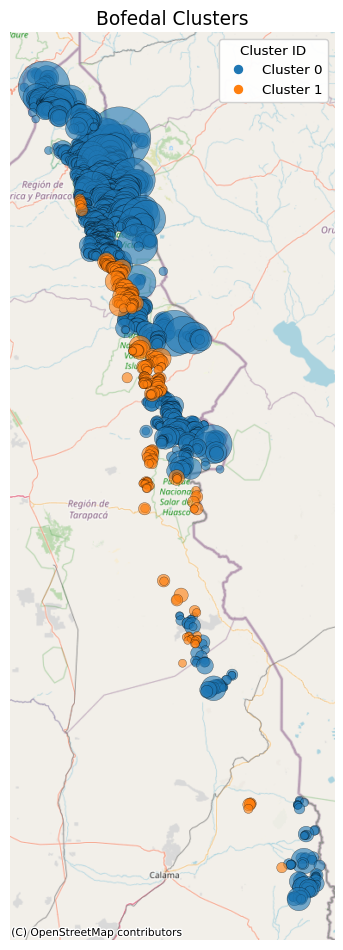
\includegraphics[keepaspectratio]{Notebooks/k2_files/figure-pdf/cell-9-output-1.png}}

\section{Feature Importance}\label{feature-importance}

\begin{Shaded}
\begin{Highlighting}[]
\NormalTok{X\_num }\OperatorTok{=}\NormalTok{ (}
\NormalTok{    df }
\NormalTok{    .select\_dtypes(}\StringTok{\textquotesingle{}number\textquotesingle{}}\NormalTok{)}
\NormalTok{    .drop(columns}\OperatorTok{=}\NormalTok{[}\StringTok{\textquotesingle{}cluster\textquotesingle{}}\NormalTok{], errors}\OperatorTok{=}\StringTok{\textquotesingle{}ignore\textquotesingle{}}\NormalTok{)}
\NormalTok{)}

\NormalTok{scaler }\OperatorTok{=}\NormalTok{ StandardScaler()}
\NormalTok{X\_scaled }\OperatorTok{=}\NormalTok{ pd.DataFrame(}
\NormalTok{    scaler.fit\_transform(X\_num),}
\NormalTok{    columns}\OperatorTok{=}\NormalTok{X\_num.columns, }
\NormalTok{    index}\OperatorTok{=}\NormalTok{X\_num.index}
\NormalTok{)}

\NormalTok{pca }\OperatorTok{=}\NormalTok{ PCA(n\_components}\OperatorTok{=}\DecValTok{6}\NormalTok{, svd\_solver}\OperatorTok{=}\StringTok{\textquotesingle{}full\textquotesingle{}}\NormalTok{).fit(X\_scaled)}

\NormalTok{pc1\_loadings }\OperatorTok{=}\NormalTok{ pd.Series(}
\NormalTok{    pca.components\_[}\DecValTok{0}\NormalTok{],}
\NormalTok{    index}\OperatorTok{=}\NormalTok{X\_scaled.columns,}
\NormalTok{    name}\OperatorTok{=}\StringTok{\textquotesingle{}PC1 loading\textquotesingle{}}
\NormalTok{)}

\BuiltInTok{print}\NormalTok{(pc1\_loadings.sort\_values(key}\OperatorTok{=}\NormalTok{np.}\BuiltInTok{abs}\NormalTok{, ascending}\OperatorTok{=}\VariableTok{False}\NormalTok{).head(}\DecValTok{20}\NormalTok{))}
\end{Highlighting}
\end{Shaded}

\begin{verbatim}
Temp Max 2004-09-01    0.024813
Temp Max 1981-09-01    0.024785
Temp Max 1997-09-01    0.024768
Temp Max 1997-08-01    0.024747
Temp Max 1982-09-01    0.024742
Temp Max 2013-01-01    0.024735
Temp Max 1993-01-01    0.024733
Temp Max 2015-01-01    0.024730
Temp Max 1979-01-01    0.024713
Temp Max 2004-08-01    0.024706
Temp Max 1987-01-01    0.024690
Temp Max 2001-01-01    0.024690
Temp Max 2005-02-01    0.024681
Temp Max 2011-05-01    0.024677
Temp Max 2008-01-01    0.024676
Temp Max 1994-09-01    0.024675
Temp Max 1992-01-01    0.024672
Temp Max 2001-08-01    0.024669
Temp Max 1997-04-01    0.024662
Temp Max 2003-09-01    0.024662
Name: PC1 loading, dtype: float64
\end{verbatim}

\begin{Shaded}
\begin{Highlighting}[]
\NormalTok{features }\OperatorTok{=}\NormalTok{ df.columns}
\NormalTok{families }\OperatorTok{=}\NormalTok{ \{}
    \StringTok{"NDVI"}\NormalTok{:  [c }\ControlFlowTok{for}\NormalTok{ c }\KeywordTok{in}\NormalTok{ features }\ControlFlowTok{if}\NormalTok{ c.startswith(}\StringTok{"NDVI"}\NormalTok{)],}
    \StringTok{"NDWI"}\NormalTok{:  [c }\ControlFlowTok{for}\NormalTok{ c }\KeywordTok{in}\NormalTok{ features }\ControlFlowTok{if}\NormalTok{ c.startswith(}\StringTok{"NDWI"}\NormalTok{)],}
    \StringTok{"GW\_rights"}\NormalTok{: [c }\ControlFlowTok{for}\NormalTok{ c }\KeywordTok{in}\NormalTok{ features }\ControlFlowTok{if}\NormalTok{ c.startswith(}\StringTok{"Ground Water Rights"}\NormalTok{)],}
    \StringTok{"SW\_rights"}\NormalTok{: [c }\ControlFlowTok{for}\NormalTok{ c }\KeywordTok{in}\NormalTok{ features }\ControlFlowTok{if}\NormalTok{ c.startswith(}\StringTok{"Surface Water Rights"}\NormalTok{)],}
    \StringTok{"Temperature"}\NormalTok{: [c }\ControlFlowTok{for}\NormalTok{ c }\KeywordTok{in}\NormalTok{ features }\ControlFlowTok{if}\NormalTok{ c.startswith((}\StringTok{"Temp Min"}\NormalTok{, }\StringTok{"Temp Max"}\NormalTok{))],}
    \StringTok{"PET"}\NormalTok{: [c }\ControlFlowTok{for}\NormalTok{ c }\KeywordTok{in}\NormalTok{ features }\ControlFlowTok{if}\NormalTok{ c.startswith(}\StringTok{"PET"}\NormalTok{)],}
    \StringTok{"Precipitation"}\NormalTok{: [c }\ControlFlowTok{for}\NormalTok{ c }\KeywordTok{in}\NormalTok{ features }\ControlFlowTok{if}\NormalTok{ c.startswith(}\StringTok{"Precipitation"}\NormalTok{)],}
    \StringTok{"Size"}\NormalTok{:   [}\StringTok{"Area\_m2"}\NormalTok{, }\StringTok{"AUC"}\NormalTok{],}
    \StringTok{"Elevation"}\NormalTok{: [c }\ControlFlowTok{for}\NormalTok{ c }\KeywordTok{in}\NormalTok{ features }\ControlFlowTok{if}\NormalTok{ c.startswith((}\StringTok{"elev\_std\_m"}\NormalTok{, }\StringTok{"elev\_mean\_"}\NormalTok{))],}
    \StringTok{"Boreholes"}\NormalTok{: [c }\ControlFlowTok{for}\NormalTok{ c }\KeywordTok{in}\NormalTok{ features }\ControlFlowTok{if}\NormalTok{ c.startswith(}\StringTok{"n\_wells"}\NormalTok{)],}
    \StringTok{"Protected Land"}\NormalTok{: [c }\ControlFlowTok{for}\NormalTok{ c }\KeywordTok{in}\NormalTok{ features }\ControlFlowTok{if}\NormalTok{ c.startswith(}\StringTok{"pct\_prot"}\NormalTok{)]}
\NormalTok{\}}

\NormalTok{summary }\OperatorTok{=}\NormalTok{ \{k: pc1\_loadings[fam].}\BuiltInTok{abs}\NormalTok{().}\BuiltInTok{sum}\NormalTok{() }\ControlFlowTok{for}\NormalTok{ k, fam }\KeywordTok{in}\NormalTok{ families.items()\}}
\NormalTok{pd.Series(summary).sort\_values(ascending}\OperatorTok{=}\VariableTok{False}\NormalTok{)}
\end{Highlighting}
\end{Shaded}

\begin{verbatim}
Temperature       23.424659
PET               11.547013
Precipitation      7.095087
SW_rights          1.571825
GW_rights          1.120259
NDVI               0.176790
NDWI               0.094735
Boreholes          0.020540
Elevation          0.008832
Protected Land     0.008541
Size               0.004697
dtype: float64
\end{verbatim}

\begin{Shaded}
\begin{Highlighting}[]
\NormalTok{pc1\_series }\OperatorTok{=}\NormalTok{ pd.Series(}
\NormalTok{    pca.transform(X\_scaled)[:, }\DecValTok{0}\NormalTok{],}
\NormalTok{    index}\OperatorTok{=}\NormalTok{X\_scaled.index,}
\NormalTok{    name}\OperatorTok{=}\StringTok{"PC1"}
\NormalTok{)}

\NormalTok{corrs }\OperatorTok{=}\NormalTok{ (}
\NormalTok{    X\_scaled}
\NormalTok{        .join(pc1\_series) }
\NormalTok{        .corr(method}\OperatorTok{=}\StringTok{"pearson"}\NormalTok{)}
\NormalTok{        .loc[}\StringTok{"PC1"}\NormalTok{]}
\NormalTok{        .drop(}\StringTok{"PC1"}\NormalTok{)}
\NormalTok{        .}\BuiltInTok{abs}\NormalTok{()}
\NormalTok{        .sort\_values(ascending}\OperatorTok{=}\VariableTok{False}\NormalTok{)}
\NormalTok{)}

\BuiltInTok{print}\NormalTok{(}\StringTok{"}\CharTok{\textbackslash{}n}\StringTok{Top |correlations| with PC1 (pandas{-}only):"}\NormalTok{)}
\NormalTok{display(corrs.head(}\DecValTok{20}\NormalTok{))}

\NormalTok{family\_corrs }\OperatorTok{=}\NormalTok{ (}
\NormalTok{    corrs}
\NormalTok{      .groupby(corrs.index.}\BuiltInTok{str}\NormalTok{.split().}\BuiltInTok{str}\NormalTok{[}\DecValTok{0}\NormalTok{])}
\NormalTok{      .}\BuiltInTok{sum}\NormalTok{()}
\NormalTok{      .sort\_values(ascending}\OperatorTok{=}\VariableTok{False}\NormalTok{)}
\NormalTok{)}

\BuiltInTok{print}\NormalTok{(}\StringTok{"}\CharTok{\textbackslash{}n}\StringTok{PC{-}1 |corr| summed by variable family:"}\NormalTok{)}
\NormalTok{display(family\_corrs.head(}\DecValTok{20}\NormalTok{))}
\end{Highlighting}
\end{Shaded}

\begin{verbatim}

Top |correlations| with PC1 (pandas-only):
\end{verbatim}

\begin{verbatim}
Temp Max 2004-09-01    0.996245
Temp Max 1981-09-01    0.995105
Temp Max 1997-09-01    0.994448
Temp Max 1997-08-01    0.993573
Temp Max 1982-09-01    0.993372
Temp Max 2013-01-01    0.993104
Temp Max 1993-01-01    0.993047
Temp Max 2015-01-01    0.992907
Temp Max 1979-01-01    0.992210
Temp Max 2004-08-01    0.991960
Temp Max 1987-01-01    0.991310
Temp Max 2001-01-01    0.991286
Temp Max 2005-02-01    0.990943
Temp Max 2011-05-01    0.990770
Temp Max 2008-01-01    0.990724
Temp Max 1994-09-01    0.990708
Temp Max 1992-01-01    0.990597
Temp Max 2001-08-01    0.990472
Temp Max 1997-04-01    0.990195
Temp Max 2003-09-01    0.990191
Name: PC1, dtype: float64
\end{verbatim}

\begin{verbatim}

PC-1 |corr| summed by variable family:
\end{verbatim}

\begin{verbatim}
Temp             940.498754
PET              463.611932
Precipitation    284.867326
Surface           63.108687
Ground            44.978350
NDVI               7.098089
NDWI               3.803588
n_wells            0.824699
lat                0.412471
pct_prot           0.342911
elev_mean_         0.332095
lon                0.249555
AUC                0.135419
Area_m2            0.053157
elev_std_m         0.022529
Name: PC1, dtype: float64
\end{verbatim}

Running the algorithm with k=2 seems to create clusters that depend
almost entirely on temperature, so the seperation does not seem very
meaningful.

\chapter{Running Without Temporal Data
(k=3)}\label{running-without-temporal-data-k3}

\begin{Shaded}
\begin{Highlighting}[]
\ImportTok{import}\NormalTok{ pandas }\ImportTok{as}\NormalTok{ pd}
\ImportTok{import}\NormalTok{ re}
\ImportTok{from}\NormalTok{ datetime }\ImportTok{import}\NormalTok{ datetime}
\ImportTok{import}\NormalTok{ numpy }\ImportTok{as}\NormalTok{ np}

\ImportTok{from}\NormalTok{ sklearn.cluster }\ImportTok{import}\NormalTok{ KMeans}
\ImportTok{from}\NormalTok{ sklearn.metrics }\ImportTok{import}\NormalTok{ silhouette\_score, davies\_bouldin\_score, calinski\_harabasz\_score}
\ImportTok{from}\NormalTok{ sklearn.preprocessing }\ImportTok{import}\NormalTok{ StandardScaler}

\ImportTok{import}\NormalTok{ matplotlib.pyplot }\ImportTok{as}\NormalTok{ plt}
\ImportTok{from}\NormalTok{ ipywidgets }\ImportTok{import}\NormalTok{ interact, widgets, Dropdown}
\ImportTok{import}\NormalTok{ seaborn }\ImportTok{as}\NormalTok{ sns}
\ImportTok{import}\NormalTok{ plotly.graph\_objects }\ImportTok{as}\NormalTok{ go}

\ImportTok{import}\NormalTok{ geopandas }\ImportTok{as}\NormalTok{ gpd}
\ImportTok{from}\NormalTok{ shapely.geometry }\ImportTok{import}\NormalTok{ Point}
\ImportTok{import}\NormalTok{ contextily }\ImportTok{as}\NormalTok{ ctx}
\ImportTok{from}\NormalTok{ matplotlib.lines }\ImportTok{import}\NormalTok{ Line2D}
\ImportTok{import}\NormalTok{ matplotlib.dates }\ImportTok{as}\NormalTok{ mdates}
\ImportTok{import}\NormalTok{ matplotlib.colors }\ImportTok{as}\NormalTok{ mcolors}
\ImportTok{import}\NormalTok{ matplotlib.cm }\ImportTok{as}\NormalTok{ cm}
\ImportTok{import}\NormalTok{ folium}

\ImportTok{import}\NormalTok{ plotly.express }\ImportTok{as}\NormalTok{ px}
\end{Highlighting}
\end{Shaded}

\begin{Shaded}
\begin{Highlighting}[]
\NormalTok{df }\OperatorTok{=}\NormalTok{ pd.read\_csv(}\StringTok{"bofedales{-}clean.csv"}\NormalTok{)}
\NormalTok{df.drop([}\StringTok{"Unnamed: 0"}\NormalTok{], axis}\OperatorTok{=}\DecValTok{1}\NormalTok{, inplace}\OperatorTok{=}\VariableTok{True}\NormalTok{)}
\NormalTok{df.head(}\DecValTok{1}\NormalTok{)}
\end{Highlighting}
\end{Shaded}

\begin{longtable}[]{@{}llllllllllllllllllllll@{}}
\toprule\noalign{}
& Area\_m2 & AUC & pct\_prot & elev\_mean\_ & elev\_std\_m & n\_wells &
Ground Water Rights 1966-01-01 & Ground Water Rights 1967-01-01 & Ground
Water Rights 1968-01-01 & Ground Water Rights 1969-01-01 & ... & NDWI
2019-03 & NDWI 2019-04 & NDWI 2019-05 & NDWI 2019-06 & NDWI 2019-07 &
NDWI 2019-08 & NDWI 2019-09 & NDWI 2019-10 & NDWI 2019-11 & NDWI
2019-12 \\
\midrule\noalign{}
\endhead
\bottomrule\noalign{}
\endlastfoot
0 & 6300 & 86.769539 & 0.0 & 4162.714286 & 3.953815 & 0.0 & 0.0 & 0.0 &
0.0 & 0.0 & ... & 0.03193 & 0.026136 & 0.022087 & 0.019181 & 0.023405 &
0.015355 & -0.000504 & 0.004056 & 0.014678 & 0.010436 \\
\end{longtable}

\begin{Shaded}
\begin{Highlighting}[]
\NormalTok{df.drop([}\StringTok{"lat"}\NormalTok{, }\StringTok{"lon"}\NormalTok{], axis}\OperatorTok{=}\DecValTok{1}\NormalTok{, inplace}\OperatorTok{=}\VariableTok{True}\NormalTok{)}
\end{Highlighting}
\end{Shaded}

\begin{Shaded}
\begin{Highlighting}[]
\NormalTok{AGG\_POLICY }\OperatorTok{=}\NormalTok{ \{}
    \CommentTok{\# family{-}name      how to aggregate?  ("latest"  or  "mean")}
    \StringTok{"Precipitation"}\NormalTok{:   }\StringTok{"mean"}\NormalTok{, }
    \StringTok{"PET"}\NormalTok{:             }\StringTok{"mean"}\NormalTok{,}
    \StringTok{"Temp Max"}\NormalTok{:        }\StringTok{"mean"}\NormalTok{,}
    \StringTok{"Temp Min"}\NormalTok{:        }\StringTok{"mean"}\NormalTok{,}
    \StringTok{"Surface Water Rights"}\NormalTok{: }\StringTok{"latest"}\NormalTok{, }
    \StringTok{"Ground Water Rights"}\NormalTok{:  }\StringTok{"latest"}\NormalTok{,}
    \StringTok{"NDWI"}\NormalTok{: }\StringTok{"mean"}\NormalTok{,}
    \StringTok{"NDVI"}\NormalTok{: }\StringTok{"mean"}
\NormalTok{\}}
\end{Highlighting}
\end{Shaded}

\begin{Shaded}
\begin{Highlighting}[]
\KeywordTok{def}\NormalTok{ condense\_temporal(df, policy):}
    \CommentTok{"""}
\CommentTok{    Collapse temporal columns based on \textasciigrave{}policy\textasciigrave{} dict.}
\CommentTok{    Returns a NEW DataFrame (original cols dropped, new cols added).}
\CommentTok{    """}
\NormalTok{    df }\OperatorTok{=}\NormalTok{ df.copy()}
    \ControlFlowTok{for}\NormalTok{ family, rule }\KeywordTok{in}\NormalTok{ policy.items():}
\NormalTok{        pattern }\OperatorTok{=}\NormalTok{ re.}\BuiltInTok{compile}\NormalTok{(}\VerbatimStringTok{rf"}\DecValTok{\^{}}\SpecialCharTok{\{}\NormalTok{re}\SpecialCharTok{.}\NormalTok{escape(family)}\SpecialCharTok{\}}\DecValTok{\textbackslash{}s}\VerbatimStringTok{"}\NormalTok{)}
\NormalTok{        fam\_cols }\OperatorTok{=}\NormalTok{ [c }\ControlFlowTok{for}\NormalTok{ c }\KeywordTok{in}\NormalTok{ df.columns }\ControlFlowTok{if}\NormalTok{ pattern.match(c)]}
        \ControlFlowTok{if} \KeywordTok{not}\NormalTok{ fam\_cols:}
            \BuiltInTok{print}\NormalTok{(}\SpecialStringTok{f" No columns found for family: }\SpecialCharTok{\{}\NormalTok{family}\SpecialCharTok{\}}\SpecialStringTok{"}\NormalTok{)}
            \ControlFlowTok{continue}

        \ControlFlowTok{if}\NormalTok{ rule }\OperatorTok{==} \StringTok{"mean"}\NormalTok{:}
\NormalTok{            new\_col }\OperatorTok{=}\NormalTok{ df[fam\_cols].mean(axis}\OperatorTok{=}\DecValTok{1}\NormalTok{)}
\NormalTok{            new\_name }\OperatorTok{=} \SpecialStringTok{f"}\SpecialCharTok{\{}\NormalTok{family}\SpecialCharTok{\}}\SpecialStringTok{"}
        \ControlFlowTok{elif}\NormalTok{ rule }\OperatorTok{==} \StringTok{"latest"}\NormalTok{:}
            \KeywordTok{def}\NormalTok{ \_parse\_date(col):}
\NormalTok{                s }\OperatorTok{=}\NormalTok{ col.replace(family, }\StringTok{""}\NormalTok{).strip()}
                \ControlFlowTok{try}\NormalTok{:}
                    \ControlFlowTok{return}\NormalTok{ datetime.strptime(s, }\StringTok{"\%Y{-}\%m{-}}\SpecialCharTok{\%d}\StringTok{"}\NormalTok{)}
                \ControlFlowTok{except} \PreprocessorTok{ValueError}\NormalTok{:}
                    \ControlFlowTok{return}\NormalTok{ datetime.strptime(s, }\StringTok{"\%Y{-}\%m"}\NormalTok{)}
\NormalTok{            latest\_col }\OperatorTok{=} \BuiltInTok{max}\NormalTok{(fam\_cols, key}\OperatorTok{=}\NormalTok{\_parse\_date)}
\NormalTok{            new\_col }\OperatorTok{=}\NormalTok{ df[latest\_col]}
\NormalTok{            new\_name }\OperatorTok{=} \SpecialStringTok{f"}\SpecialCharTok{\{}\NormalTok{family}\SpecialCharTok{\}}\SpecialStringTok{"}
        \ControlFlowTok{else}\NormalTok{:}
            \ControlFlowTok{raise} \PreprocessorTok{ValueError}\NormalTok{(}\SpecialStringTok{f"Unknown rule \textquotesingle{}}\SpecialCharTok{\{}\NormalTok{rule}\SpecialCharTok{\}}\SpecialStringTok{\textquotesingle{} for }\SpecialCharTok{\{}\NormalTok{family}\SpecialCharTok{\}}\SpecialStringTok{"}\NormalTok{)}

\NormalTok{        df[new\_name] }\OperatorTok{=}\NormalTok{ new\_col}
\NormalTok{        df }\OperatorTok{=}\NormalTok{ df.drop(columns}\OperatorTok{=}\NormalTok{fam\_cols)}

    \ControlFlowTok{return}\NormalTok{ df}
\end{Highlighting}
\end{Shaded}

\begin{Shaded}
\begin{Highlighting}[]
\NormalTok{df\_condensed }\OperatorTok{=}\NormalTok{ condense\_temporal(df, AGG\_POLICY)}

\NormalTok{df\_condensed }\OperatorTok{=}\NormalTok{ df\_condensed.rename(columns}\OperatorTok{=}\NormalTok{\{}\StringTok{\textquotesingle{}pct\_prot\textquotesingle{}}\NormalTok{: }\StringTok{\textquotesingle{}Percentage Protected Land (of total bofedal)\textquotesingle{}}\NormalTok{, }
                        \StringTok{\textquotesingle{}Area\_m2\textquotesingle{}}\NormalTok{: }\StringTok{\textquotesingle{}Area (m²)\textquotesingle{}}\NormalTok{, }
                        \StringTok{\textquotesingle{}AUC\textquotesingle{}}\NormalTok{: }\StringTok{\textquotesingle{}Area of basin\textquotesingle{}}\NormalTok{, }
                        \StringTok{\textquotesingle{}elev\_mean\_\textquotesingle{}}\NormalTok{: }\StringTok{\textquotesingle{}Average Elevation (m)\textquotesingle{}}\NormalTok{,}
                        \StringTok{\textquotesingle{}elev\_std\_m\textquotesingle{}}\NormalTok{: }\StringTok{\textquotesingle{}Elevation Standard Deviation (m)\textquotesingle{}}\NormalTok{,}
                        \StringTok{\textquotesingle{}n\_wells\textquotesingle{}}\NormalTok{: }\StringTok{\textquotesingle{}Number of wells (per catchment area)\textquotesingle{}}\NormalTok{,}
                        \StringTok{\textquotesingle{}Precipitation\textquotesingle{}}\NormalTok{: }\StringTok{\textquotesingle{}Precipitation (mm)\textquotesingle{}}\NormalTok{,}
                        \StringTok{\textquotesingle{}PET\textquotesingle{}}\NormalTok{: }\StringTok{\textquotesingle{}PET (mm)\textquotesingle{}}\NormalTok{,}
                        \StringTok{\textquotesingle{}Temp Max\textquotesingle{}}\NormalTok{: }\StringTok{\textquotesingle{}Maximum Temperature (°C)\textquotesingle{}}\NormalTok{,}
                        \StringTok{\textquotesingle{}Temp Min\textquotesingle{}}\NormalTok{: }\StringTok{\textquotesingle{}Minimum Temperature (°C)\textquotesingle{}}\NormalTok{,}
                        \StringTok{\textquotesingle{}Surface Water Rights\textquotesingle{}}\NormalTok{: }\StringTok{\textquotesingle{}Surface Water Rights (L/s)\textquotesingle{}}\NormalTok{,}
                        \StringTok{\textquotesingle{}Ground Water Rights\textquotesingle{}}\NormalTok{: }\StringTok{\textquotesingle{}Ground Water Rights (L/s)\textquotesingle{}}\NormalTok{,}
\NormalTok{                    \})}

\NormalTok{features\_df }\OperatorTok{=}\NormalTok{ (}
\NormalTok{    df\_condensed}
\NormalTok{    .select\_dtypes(}\StringTok{"number"}\NormalTok{)}
\NormalTok{    .drop(columns}\OperatorTok{=}\NormalTok{[}\StringTok{"cluster"}\NormalTok{], errors}\OperatorTok{=}\StringTok{"ignore"}\NormalTok{)}
\NormalTok{)}

\NormalTok{scaler }\OperatorTok{=}\NormalTok{ StandardScaler()}
\NormalTok{X\_scaled }\OperatorTok{=}\NormalTok{ scaler.fit\_transform(features\_df)}
\end{Highlighting}
\end{Shaded}

\begin{Shaded}
\begin{Highlighting}[]
\KeywordTok{def}\NormalTok{ kmeans\_diagnostics(}
\NormalTok{        features\_df,}
\NormalTok{        k\_range}\OperatorTok{=}\BuiltInTok{range}\NormalTok{(}\DecValTok{2}\NormalTok{, }\DecValTok{11}\NormalTok{),}
\NormalTok{        scaler}\OperatorTok{=}\VariableTok{None}\NormalTok{,}
\NormalTok{        random\_state}\OperatorTok{=}\DecValTok{0}
\NormalTok{    ):}
    \CommentTok{"""}
\CommentTok{    Runs KMeans for each k in k\_range, computes cluster{-}validity metrics,}
\CommentTok{    makes diagnostic plots, and returns a DataFrame of the results.}
\CommentTok{    """}
\NormalTok{    X }\OperatorTok{=}\NormalTok{ features\_df.select\_dtypes(}\StringTok{\textquotesingle{}number\textquotesingle{}}\NormalTok{).copy()}
    
\NormalTok{    scaler }\OperatorTok{=}\NormalTok{ scaler }\KeywordTok{or}\NormalTok{ StandardScaler()}
\NormalTok{    X\_scaled }\OperatorTok{=}\NormalTok{ scaler.fit\_transform(X)}

\NormalTok{    inertias, sils, dbs, chs }\OperatorTok{=}\NormalTok{ [], [], [], []}

    \ControlFlowTok{for}\NormalTok{ k }\KeywordTok{in}\NormalTok{ k\_range:}
\NormalTok{        km }\OperatorTok{=}\NormalTok{ KMeans(n\_clusters}\OperatorTok{=}\NormalTok{k, random\_state}\OperatorTok{=}\NormalTok{random\_state, n\_init}\OperatorTok{=}\StringTok{"auto"}\NormalTok{)}
\NormalTok{        labels }\OperatorTok{=}\NormalTok{ km.fit\_predict(X\_scaled)}

\NormalTok{        inertias.append(km.inertia\_)}
\NormalTok{        sils.append(silhouette\_score(X\_scaled, labels))}
\NormalTok{        dbs.append(davies\_bouldin\_score(X\_scaled, labels))}
\NormalTok{        chs.append(calinski\_harabasz\_score(X\_scaled, labels))}

\NormalTok{    fig, axes }\OperatorTok{=}\NormalTok{ plt.subplots(}\DecValTok{1}\NormalTok{, }\DecValTok{2}\NormalTok{, figsize}\OperatorTok{=}\NormalTok{(}\DecValTok{12}\NormalTok{, }\DecValTok{4}\NormalTok{))}
    
\NormalTok{    axes[}\DecValTok{0}\NormalTok{].plot(k\_range, inertias, }\StringTok{"o{-}"}\NormalTok{)}
\NormalTok{    axes[}\DecValTok{0}\NormalTok{].}\BuiltInTok{set}\NormalTok{(}
\NormalTok{        xlabel}\OperatorTok{=}\StringTok{"k (clusters)"}\NormalTok{,}
\NormalTok{        ylabel}\OperatorTok{=}\StringTok{"Inertia (WCSS)"}\NormalTok{,}
\NormalTok{        title}\OperatorTok{=}\StringTok{"Elbow method"}
\NormalTok{    )}
    
\NormalTok{    axes[}\DecValTok{1}\NormalTok{].plot(k\_range, sils, }\StringTok{"o{-}"}\NormalTok{, label}\OperatorTok{=}\StringTok{"Silhouette ↑"}\NormalTok{)}
\NormalTok{    axes[}\DecValTok{1}\NormalTok{].plot(k\_range, dbs,  }\StringTok{"o{-}"}\NormalTok{, label}\OperatorTok{=}\StringTok{"Davies–Bouldin ↓"}\NormalTok{)}
\NormalTok{    axes[}\DecValTok{1}\NormalTok{].plot(k\_range, chs,  }\StringTok{"o{-}"}\NormalTok{, label}\OperatorTok{=}\StringTok{"Calinski–Harabasz ↑"}\NormalTok{)}
\NormalTok{    axes[}\DecValTok{1}\NormalTok{].}\BuiltInTok{set}\NormalTok{(}
\NormalTok{        xlabel}\OperatorTok{=}\StringTok{"k (clusters)"}\NormalTok{,}
\NormalTok{        title}\OperatorTok{=}\StringTok{"Cluster{-}validity indices"}
\NormalTok{    )}
\NormalTok{    axes[}\DecValTok{1}\NormalTok{].legend()}
\NormalTok{    plt.tight\_layout()}
\NormalTok{    plt.show()}

\NormalTok{    metrics }\OperatorTok{=}\NormalTok{ pd.DataFrame(\{}
        \StringTok{"k"}\NormalTok{: }\BuiltInTok{list}\NormalTok{(k\_range),}
        \StringTok{"inertia"}\NormalTok{: inertias,}
        \StringTok{"silhouette"}\NormalTok{: sils,}
        \StringTok{"davies\_bouldin"}\NormalTok{: dbs,}
        \StringTok{"calinski\_harabasz"}\NormalTok{: chs}
\NormalTok{    \})}
    \ControlFlowTok{return}\NormalTok{ metrics}

\NormalTok{metrics }\OperatorTok{=}\NormalTok{ kmeans\_diagnostics(}
\NormalTok{    features\_df,}
\NormalTok{    k\_range}\OperatorTok{=}\BuiltInTok{range}\NormalTok{(}\DecValTok{2}\NormalTok{, }\DecValTok{11}\NormalTok{), }
\NormalTok{    random\_state}\OperatorTok{=}\DecValTok{42}
\NormalTok{)}

\NormalTok{display(metrics.sort\_values(}\StringTok{"silhouette"}\NormalTok{, ascending}\OperatorTok{=}\VariableTok{False}\NormalTok{))}
\end{Highlighting}
\end{Shaded}

\pandocbounded{\includegraphics[keepaspectratio]{Notebooks/k3_files/figure-pdf/cell-8-output-1.png}}

\begin{longtable}[]{@{}llllll@{}}
\toprule\noalign{}
& k & inertia & silhouette & davies\_bouldin & calinski\_harabasz \\
\midrule\noalign{}
\endhead
\bottomrule\noalign{}
\endlastfoot
0 & 2 & 24487.019836 & 0.567626 & 0.561799 & 1136.279464 \\
1 & 3 & 18113.360620 & 0.323346 & 1.113283 & 1213.057466 \\
2 & 4 & 15573.777886 & 0.312550 & 1.309326 & 1077.738599 \\
3 & 5 & 14130.147582 & 0.283505 & 1.341564 & 955.114949 \\
7 & 9 & 9894.428930 & 0.274834 & 1.247715 & 816.033288 \\
6 & 8 & 10458.801158 & 0.270735 & 1.232154 & 863.161538 \\
5 & 7 & 12153.917345 & 0.261101 & 1.425589 & 808.174314 \\
4 & 6 & 13983.328016 & 0.256730 & 1.605868 & 777.117932 \\
8 & 10 & 9747.609364 & 0.250140 & 1.413670 & 740.220904 \\
\end{longtable}

Due to the above metrics, we use k=3 for the algorithm

\begin{Shaded}
\begin{Highlighting}[]
\NormalTok{k}\OperatorTok{=}\DecValTok{3}
\NormalTok{kmeans }\OperatorTok{=}\NormalTok{ KMeans(n\_clusters}\OperatorTok{=}\NormalTok{k, random\_state}\OperatorTok{=}\DecValTok{0}\NormalTok{, n\_init}\OperatorTok{=}\StringTok{"auto"}\NormalTok{).fit(X\_scaled)}
\NormalTok{df\_condensed[}\StringTok{"cluster"}\NormalTok{] }\OperatorTok{=}\NormalTok{ kmeans.labels\_}
\NormalTok{df\_condensed.head(}\DecValTok{3}\NormalTok{)}
\end{Highlighting}
\end{Shaded}

\begin{longtable}[]{@{}llllllllllllllll@{}}
\toprule\noalign{}
& Area (m²) & Area of basin & Percentage Protected Land (of total
bofedal) & Average Elevation (m) & Elevation Standard Deviation (m) &
Number of wells (per catchment area) & Precipitation (mm) & PET (mm) &
Maximum Temperature (°C) & Minimum Temperature (°C) & Surface Water
Rights (L/s) & Ground Water Rights (L/s) & NDWI & NDVI & cluster \\
\midrule\noalign{}
\endhead
\bottomrule\noalign{}
\endlastfoot
0 & 6300 & 86.769539 & 0.0 & 4162.714286 & 3.953815 & 0.0 & 15.011753 &
76.43679 & 9.74673 & -5.034592 & 1715.5 & 2424.3 & -0.003601 & 0.218041
& 1 \\
1 & 5400 & 83.176353 & 0.0 & 4073.500000 & 12.406316 & 0.0 & 15.011753 &
76.43679 & 9.74673 & -5.034592 & 1715.5 & 2424.3 & -0.046695 & 0.205608
& 1 \\
2 & 6300 & 103.719438 & 0.0 & 4278.571429 & 6.161102 & 0.0 & 15.011753 &
76.43679 & 9.74673 & -5.034592 & 1715.5 & 2424.3 & 0.035979 & 0.180369 &
1 \\
\end{longtable}

\begin{Shaded}
\begin{Highlighting}[]
\NormalTok{sns.pairplot(}
\NormalTok{    df\_condensed.assign(cluster}\OperatorTok{=}\NormalTok{kmeans.labels\_),}
    \BuiltInTok{vars}\OperatorTok{=}\NormalTok{[}\StringTok{"Maximum Temperature (°C)"}\NormalTok{, }\StringTok{"Precipitation (mm)"}\NormalTok{, }\StringTok{"PET (mm)"}\NormalTok{],}
\NormalTok{    hue}\OperatorTok{=}\StringTok{"cluster"}\NormalTok{, palette}\OperatorTok{=}\StringTok{"Set2"}
\NormalTok{)}\OperatorTok{;}\NormalTok{ plt.show()}

\NormalTok{centroids }\OperatorTok{=}\NormalTok{ pd.DataFrame(kmeans.cluster\_centers\_, columns}\OperatorTok{=}\NormalTok{features\_df.columns)}
\BuiltInTok{print}\NormalTok{(}\StringTok{"}\CharTok{\textbackslash{}n}\StringTok{Centroid means (k = 3):"}\NormalTok{)}
\NormalTok{display(centroids.T)}
\end{Highlighting}
\end{Shaded}

\pandocbounded{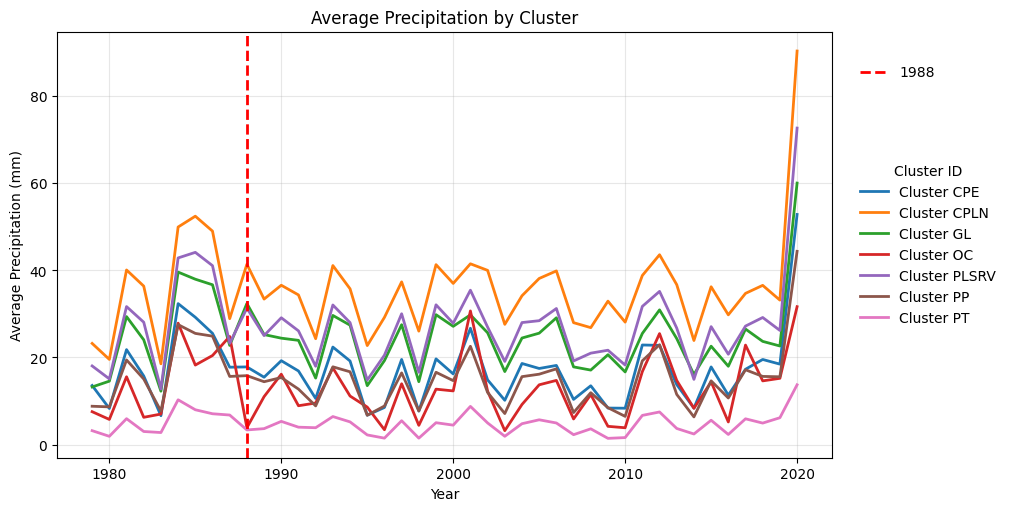
\includegraphics[keepaspectratio]{Notebooks/k3_files/figure-pdf/cell-10-output-1.png}}

\begin{verbatim}

Centroid means (k = 3):
\end{verbatim}

\begin{longtable}[]{@{}llll@{}}
\toprule\noalign{}
& 0 & 1 & 2 \\
\midrule\noalign{}
\endhead
\bottomrule\noalign{}
\endlastfoot
Area (m²) & -0.002319 & 0.013485 & -0.094332 \\
Area of basin & -0.351732 & 0.279181 & 0.028752 \\
Percentage Protected Land (of total bofedal) & 0.931268 & -0.680084 &
-0.555803 \\
Average Elevation (m) & 0.495675 & -0.304058 & -0.766003 \\
Elevation Standard Deviation (m) & -0.110698 & 0.100587 & -0.094223 \\
Number of wells (per catchment area) & -0.266041 & -0.254487 &
3.801576 \\
Precipitation (mm) & 0.786080 & -0.356371 & -2.236167 \\
PET (mm) & -0.371031 & -0.126565 & 3.448225 \\
Maximum Temperature (°C) & -0.461297 & -0.032838 & 3.276376 \\
Minimum Temperature (°C) & -0.807797 & 0.357518 & 2.368550 \\
Surface Water Rights (L/s) & 1.095665 & -0.810426 & -0.570421 \\
Ground Water Rights (L/s) & -0.257634 & -0.263003 & 3.815851 \\
NDWI & -0.341034 & 0.285102 & -0.089108 \\
NDVI & -0.283815 & 0.231884 & -0.030463 \\
\end{longtable}

\subsubsection{Results}\label{results}

\begin{itemize}
\tightlist
\item
  Cluster 0: Cool \& wet bofedales
\item
  Cluster 1: Moderate sites balancing both factors
\item
  Cluster 2: Hot \& extremely dry outliers
\end{itemize}

\begin{Shaded}
\begin{Highlighting}[]
\NormalTok{df\_condensed[}\StringTok{"lat"}\NormalTok{] }\OperatorTok{=}\NormalTok{ pd.read\_csv(}\StringTok{"bofedales{-}clean.csv"}\NormalTok{)[}\StringTok{"lat"}\NormalTok{]}
\NormalTok{df\_condensed[}\StringTok{"lon"}\NormalTok{] }\OperatorTok{=}\NormalTok{ pd.read\_csv(}\StringTok{"bofedales{-}clean.csv"}\NormalTok{)[}\StringTok{"lon"}\NormalTok{]}
\NormalTok{df }\OperatorTok{=}\NormalTok{ df\_condensed}
\end{Highlighting}
\end{Shaded}

\begin{Shaded}
\begin{Highlighting}[]
\NormalTok{geometry }\OperatorTok{=}\NormalTok{ [Point(xy) }\ControlFlowTok{for}\NormalTok{ xy }\KeywordTok{in} \BuiltInTok{zip}\NormalTok{(df.lon, df.lat)]}

\NormalTok{gdf }\OperatorTok{=}\NormalTok{ gpd.GeoDataFrame(}
\NormalTok{    df.copy(), }
\NormalTok{    geometry}\OperatorTok{=}\NormalTok{geometry,}
\NormalTok{    crs}\OperatorTok{=}\StringTok{"EPSG:4326"}
\NormalTok{)}

\NormalTok{gdf[}\StringTok{"size\_for\_plot"}\NormalTok{] }\OperatorTok{=}\NormalTok{ gdf[}\StringTok{"Area (m²)"}\NormalTok{].}\BuiltInTok{apply}\NormalTok{(}\KeywordTok{lambda}\NormalTok{ a: (a}\OperatorTok{**}\FloatTok{0.5}\NormalTok{))}

\NormalTok{scale\_factor }\OperatorTok{=} \FloatTok{0.5}
\NormalTok{gdf[}\StringTok{"size\_for\_plot"}\NormalTok{] }\OperatorTok{*=}\NormalTok{ scale\_factor}

\NormalTok{gdf\_3857 }\OperatorTok{=}\NormalTok{ gdf.to\_crs(epsg}\OperatorTok{=}\DecValTok{3857}\NormalTok{)}
\NormalTok{fig, ax }\OperatorTok{=}\NormalTok{ plt.subplots(figsize}\OperatorTok{=}\NormalTok{(}\DecValTok{8}\NormalTok{, }\DecValTok{10}\NormalTok{))}

\NormalTok{cmap }\OperatorTok{=}\NormalTok{ plt.get\_cmap(}\StringTok{"tab10"}\NormalTok{)}

\ControlFlowTok{for}\NormalTok{ i, cluster\_id }\KeywordTok{in} \BuiltInTok{enumerate}\NormalTok{(}\BuiltInTok{sorted}\NormalTok{(gdf\_3857[}\StringTok{"cluster"}\NormalTok{].unique())):}
\NormalTok{    subset }\OperatorTok{=}\NormalTok{ gdf\_3857[gdf\_3857[}\StringTok{"cluster"}\NormalTok{] }\OperatorTok{==}\NormalTok{ cluster\_id]}
    
\NormalTok{    ax.scatter(}
\NormalTok{        subset.geometry.x,}
\NormalTok{        subset.geometry.y,}
\NormalTok{        s}\OperatorTok{=}\NormalTok{subset[}\StringTok{"size\_for\_plot"}\NormalTok{],}
\NormalTok{        c}\OperatorTok{=}\NormalTok{[cmap(i)],}
\NormalTok{        alpha}\OperatorTok{=}\FloatTok{0.6}\NormalTok{,}
\NormalTok{        edgecolor}\OperatorTok{=}\StringTok{"k"}\NormalTok{,}
\NormalTok{        linewidth}\OperatorTok{=}\FloatTok{0.3}\NormalTok{,}
\NormalTok{        label}\OperatorTok{=}\SpecialStringTok{f"Cluster }\SpecialCharTok{\{}\NormalTok{cluster\_id}\SpecialCharTok{\}}\SpecialStringTok{"}
\NormalTok{    )}

\NormalTok{ctx.add\_basemap(}
\NormalTok{    ax,}
\NormalTok{    source}\OperatorTok{=}\NormalTok{ctx.providers.OpenStreetMap.Mapnik,}
\NormalTok{)}

\NormalTok{cluster\_handles }\OperatorTok{=}\NormalTok{ []}
\ControlFlowTok{for}\NormalTok{ idx, cluster\_id }\KeywordTok{in} \BuiltInTok{enumerate}\NormalTok{(}\BuiltInTok{sorted}\NormalTok{(gdf\_3857[}\StringTok{"cluster"}\NormalTok{].unique())):}
\NormalTok{    cluster\_handles.append(}
\NormalTok{        Line2D(}
\NormalTok{            [], [], }
\NormalTok{            marker}\OperatorTok{=}\StringTok{"o"}\NormalTok{, }
\NormalTok{            markersize}\OperatorTok{=}\DecValTok{6}\NormalTok{, }
\NormalTok{            color}\OperatorTok{=}\NormalTok{cmap(idx),}
\NormalTok{            linestyle}\OperatorTok{=}\StringTok{""}\NormalTok{,}
\NormalTok{            label}\OperatorTok{=}\SpecialStringTok{f"Cluster }\SpecialCharTok{\{}\NormalTok{cluster\_id}\SpecialCharTok{\}}\SpecialStringTok{"}\NormalTok{,}
\NormalTok{        )}
\NormalTok{    )}

\NormalTok{legend1 }\OperatorTok{=}\NormalTok{ ax.legend(handles}\OperatorTok{=}\NormalTok{cluster\_handles, title}\OperatorTok{=}\StringTok{"Cluster ID"}\NormalTok{, loc}\OperatorTok{=}\StringTok{"upper right"}\NormalTok{)}
\NormalTok{ax.add\_artist(legend1)}

\NormalTok{ax.set\_aspect(}\StringTok{\textquotesingle{}equal\textquotesingle{}}\NormalTok{, adjustable}\OperatorTok{=}\StringTok{\textquotesingle{}box\textquotesingle{}}\NormalTok{)}

\NormalTok{ax.set\_axis\_off()}
\NormalTok{ax.set\_title(}\StringTok{"Bofedal Clusters"}\NormalTok{, fontsize}\OperatorTok{=}\DecValTok{14}\NormalTok{)}
\NormalTok{plt.tight\_layout()}
\NormalTok{plt.show()}
\end{Highlighting}
\end{Shaded}

\pandocbounded{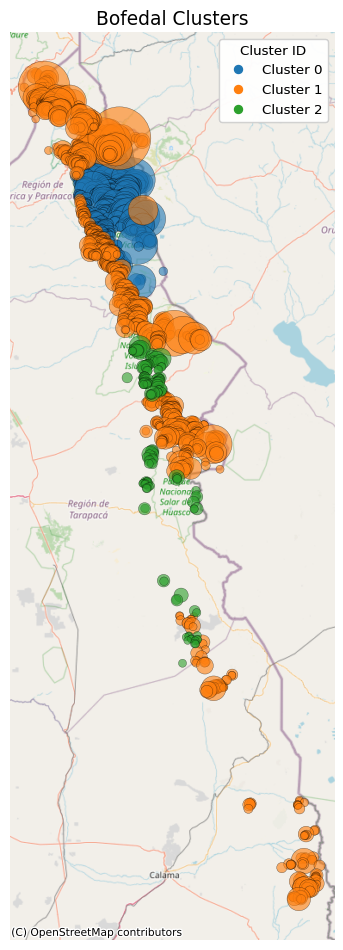
\includegraphics[keepaspectratio]{Notebooks/k3_files/figure-pdf/cell-12-output-1.png}}

\begin{Shaded}
\begin{Highlighting}[]
\NormalTok{palette }\OperatorTok{=}\NormalTok{ [}
    \StringTok{"indianred"}\NormalTok{,}\StringTok{"lightsalmon"}\NormalTok{,}\StringTok{"mediumaquamarine"}\NormalTok{,}\StringTok{"powderblue"}\NormalTok{,}\StringTok{"darkslateblue"}\NormalTok{,}
    \StringTok{"mediumturquoise"}\NormalTok{,}\StringTok{"lavender"}\NormalTok{,}\StringTok{"palevioletred"}\NormalTok{,}\StringTok{"olivedrab"}\NormalTok{,}\StringTok{"lightpink"}\NormalTok{,}
    \StringTok{"gold"}\NormalTok{,}\StringTok{"mediumvioletred"}\NormalTok{,}\StringTok{"lightcoral"}\NormalTok{,}\StringTok{"tomato"}\NormalTok{,}\StringTok{"sandybrown"}\NormalTok{,}
    \StringTok{"darkseagreen"}\NormalTok{,}\StringTok{"lemonchiffon"}\NormalTok{,}\StringTok{"darksalmon"}\NormalTok{,}\StringTok{"darkred"}\NormalTok{,}\StringTok{"firebrick"}\NormalTok{,}
    \StringTok{"oldlace"}\NormalTok{,}\StringTok{"royalblue"}\NormalTok{,}\StringTok{"mediumpurple"}\NormalTok{,}\StringTok{"plum"}
\NormalTok{]}

\NormalTok{agg }\OperatorTok{=}\NormalTok{ (df\_condensed}
\NormalTok{       .groupby(}\StringTok{"cluster"}\NormalTok{)}
\NormalTok{       .mean()}
\NormalTok{       .reset\_index())}


\KeywordTok{def}\NormalTok{ make\_trace(var, colour):}
    \ControlFlowTok{return}\NormalTok{ go.Bar(}
\NormalTok{        x}\OperatorTok{=}\NormalTok{agg[}\StringTok{"cluster"}\NormalTok{].astype(}\BuiltInTok{str}\NormalTok{),}
\NormalTok{        y}\OperatorTok{=}\NormalTok{agg[var],}
\NormalTok{        marker}\OperatorTok{=}\BuiltInTok{dict}\NormalTok{(color}\OperatorTok{=}\NormalTok{colour, line}\OperatorTok{=}\BuiltInTok{dict}\NormalTok{(color}\OperatorTok{=}\StringTok{"black"}\NormalTok{)),}
\NormalTok{        name}\OperatorTok{=}\NormalTok{var}
\NormalTok{    )}

\NormalTok{vars\_list }\OperatorTok{=} \BuiltInTok{list}\NormalTok{(agg.columns[}\DecValTok{1}\NormalTok{:])}
\NormalTok{default\_var }\OperatorTok{=}\NormalTok{ vars\_list[}\DecValTok{0}\NormalTok{]}

\NormalTok{fig }\OperatorTok{=}\NormalTok{ go.Figure(make\_trace(default\_var, palette[}\DecValTok{0}\NormalTok{]))}

\NormalTok{buttons }\OperatorTok{=}\NormalTok{ []}
\ControlFlowTok{for}\NormalTok{ i, var }\KeywordTok{in} \BuiltInTok{enumerate}\NormalTok{(vars\_list):}
\NormalTok{    buttons.append(}
        \BuiltInTok{dict}\NormalTok{(}
\NormalTok{            label  }\OperatorTok{=}\NormalTok{ var,}
\NormalTok{            method }\OperatorTok{=} \StringTok{"update"}\NormalTok{,}
\NormalTok{            args   }\OperatorTok{=}\NormalTok{ [}
\NormalTok{                \{}\StringTok{"y"}\NormalTok{: [agg[var]],}
                 \StringTok{"marker.color"}\NormalTok{: [palette[i }\OperatorTok{\%} \BuiltInTok{len}\NormalTok{(palette)]]\},}
\NormalTok{                \{}
                  \StringTok{"title"}\NormalTok{: }\SpecialStringTok{f"Average }\SpecialCharTok{\{}\NormalTok{var}\SpecialCharTok{\}}\SpecialStringTok{ per cluster"}\NormalTok{,}
                  \StringTok{"yaxis"}\NormalTok{: \{}\StringTok{"title"}\NormalTok{: \{}\StringTok{"text"}\NormalTok{: var\}\}}
\NormalTok{                \}}
\NormalTok{            ]}
\NormalTok{        )}
\NormalTok{    )}

\NormalTok{fig.update\_layout(}
\NormalTok{    yaxis\_title}\OperatorTok{=}\NormalTok{default\_var,}
\NormalTok{    xaxis}\OperatorTok{=}\BuiltInTok{dict}\NormalTok{(title}\OperatorTok{=}\StringTok{"Cluster"}\NormalTok{, }\BuiltInTok{type}\OperatorTok{=}\StringTok{"category"}\NormalTok{),}
\NormalTok{    updatemenus}\OperatorTok{=}\NormalTok{[}\BuiltInTok{dict}\NormalTok{(}
        \BuiltInTok{type}\OperatorTok{=}\StringTok{"dropdown"}\NormalTok{,}
\NormalTok{        direction}\OperatorTok{=}\StringTok{"down"}\NormalTok{,}
\NormalTok{        showactive}\OperatorTok{=}\VariableTok{True}\NormalTok{,}
\NormalTok{        buttons}\OperatorTok{=}\NormalTok{buttons,}
\NormalTok{        x}\OperatorTok{=}\FloatTok{0.0}\NormalTok{, xanchor}\OperatorTok{=}\StringTok{"left"}\NormalTok{,}
\NormalTok{        y}\OperatorTok{=}\FloatTok{1.15}\NormalTok{, yanchor}\OperatorTok{=}\StringTok{"top"}
\NormalTok{    )],}
\NormalTok{    margin}\OperatorTok{=}\BuiltInTok{dict}\NormalTok{(t}\OperatorTok{=}\DecValTok{90}\NormalTok{, r}\OperatorTok{=}\DecValTok{20}\NormalTok{, l}\OperatorTok{=}\DecValTok{60}\NormalTok{, b}\OperatorTok{=}\DecValTok{50}\NormalTok{),}
\NormalTok{    height}\OperatorTok{=}\DecValTok{450}\NormalTok{, width}\OperatorTok{=}\DecValTok{700}\NormalTok{,}
\NormalTok{    showlegend}\OperatorTok{=}\VariableTok{False}
\NormalTok{)}

\NormalTok{fig}
\end{Highlighting}
\end{Shaded}

\begin{verbatim}
Unable to display output for mime type(s): text/html
\end{verbatim}

\begin{verbatim}
Unable to display output for mime type(s): text/html
\end{verbatim}




\end{document}
